%% Evaluation Protocol Outweighs Multimodal Fusion in Wearable and Camera-Based
%% Stress and Attention Monitoring: A Systematic Review with Within-Study Meta-Analysis
%%
%% Self-contained LaTeX source. Compile with:
%%     pdflatex Manuscript_BSPC.tex && pdflatex Manuscript_BSPC.tex
%% Requires: texlive-latex-extra, texlive-pictures, texlive-fonts-recommended.
%% Keep the figures/ directory alongside this file (Overleaf: upload the
%% supplied Overleaf zip with "New Project > Upload Project", which already
%% contains this .tex plus the figures/ folder).

\documentclass[11pt,a4paper]{article}
\usepackage[margin=0.7in]{geometry}
\usepackage[T1]{fontenc}
\usepackage[utf8]{inputenc}
\usepackage{times}
\usepackage{amsmath,amssymb}
\usepackage{graphicx}
\graphicspath{{figures/}{./}{../figures/}}
\usepackage{booktabs}
\usepackage{longtable}
\usepackage{tabularx}
\usepackage{array}
\usepackage{multirow}
\usepackage{caption}
\usepackage{float}
\usepackage{enumitem}
\usepackage[table]{xcolor}
\usepackage{tikz}
\usepackage{titlesec}
\usepackage[hidelinks]{hyperref}
\usetikzlibrary{shapes.geometric,arrows.meta,positioning,calc,fit,backgrounds}

\captionsetup{font=small,labelfont=bf,labelsep=colon,justification=justified,
              singlelinecheck=false,skip=5pt}
\captionsetup[table]{position=above}
\setlength{\parskip}{4pt}
\setlength{\parindent}{0pt}
\renewcommand{\arraystretch}{1.14}
\setlength{\tabcolsep}{4pt}
\titleformat{\section}{\normalfont\large\bfseries}{\thesection.}{0.6em}{}
\titleformat{\subsection}{\normalfont\normalsize\bfseries}{\thesubsection}{0.6em}{}
\titleformat{\subsubsection}{\normalfont\normalsize\itshape}{\thesubsubsection}{0.6em}{}
\titlespacing*{\section}{0pt}{12pt}{5pt}
\titlespacing*{\subsection}{0pt}{9pt}{3pt}
\titlespacing*{\subsubsection}{0pt}{7pt}{2pt}

\definecolor{hdr}{HTML}{E8EDF3}
\definecolor{acc}{HTML}{2B6CB0}
\definecolor{wrn}{HTML}{C53030}
\definecolor{soft}{HTML}{F5F7FA}
\newcolumntype{L}[1]{>{\raggedright\arraybackslash}p{#1}}
\newcolumntype{C}[1]{>{\centering\arraybackslash}p{#1}}

\tikzset{
  blk/.style={rectangle,rounded corners=2pt,draw=acc!80,fill=acc!8,line width=0.7pt,
              align=center,inner sep=4pt,font=\scriptsize,minimum height=8.5mm},
  sens/.style={blk,fill=green!7,draw=green!45!black},
  proc/.style={blk,fill=orange!8,draw=orange!65!black},
  fuse/.style={blk,fill=purple!8,draw=purple!60!black},
  outp/.style={blk,fill=red!6,draw=red!60!black},
  pr/.style={rectangle,draw=black!65,line width=0.6pt,align=left,inner sep=4pt,
             font=\scriptsize,text width=62mm,fill=soft},
  prx/.style={pr,text width=66mm,fill=white},
  ar/.style={-{Latex[length=2mm,width=1.4mm]},line width=0.6pt,draw=black!70},
}

\begin{document}
\thispagestyle{empty}
\begin{center}
{\bfseries\large Title Page (with author details)}\\[14pt]
{\large\bfseries Evaluation Protocol Outweighs Multimodal Fusion in Wearable Stress and\\[2pt]
Attention Monitoring: Systematic Review and Meta-Analysis}\\[14pt]
\end{center}

Alvi Ibn Amzad Anil\textsuperscript{1}, Abtahi Noor\textsuperscript{1},
Md Saif Kabir\textsuperscript{1*}, Mohammad Fahim\textsuperscript{2},
Md. Mehedi Hasan Shawon\textsuperscript{2}, Sumaiya Akter\textsuperscript{2},
Md. Golam Rabiul Alam\textsuperscript{2}

\vspace{6pt}
\textsuperscript{1}Department of Electrical and Electronic Engineering, BSRM School of
Engineering, BRAC University, Dhaka, Bangladesh\\
\textsuperscript{2}Department of Computer Science and Engineering, School of Data and
Sciences, BRAC University, Dhaka, Bangladesh

\vspace{6pt}
alviamzad02@gmail.com, abtahinoor20@gmail.com, saif.kabir@bracu.ac.bd,
mohammad.fahim@bracu.ac.bd, shawon.cse.bracu@gmail.com,
sumaiya.akter.cse.bracu@gmail.com, rabiul.alam@bracu.ac.bd

\vspace{10pt}
\textbf{Order of Authors:} Alvi Ibn Amzad Anil; Abtahi Noor; Md Saif Kabir*;
Mohammad Fahim; Md. Mehedi Hasan Shawon; Sumaiya Akter; Md. Golam Rabiul Alam.

\vspace{10pt}
\textbf{Corresponding author:}\\
Md Saif Kabir, Senior Lecturer, Office of Academic Advising (OAA);
Adjunct Faculty, Department of Electrical and Electronic Engineering,
BSRM School of Engineering, BRAC University, Dhaka, Bangladesh.\\
Email: saif.kabir@bracu.ac.bd

\vspace{10pt}
\textbf{Author Contribution Statement:}\\
\textbf{Alvi Ibn Amzad Anil:} Conceptualization, Methodology, Software, Validation, Formal
Analysis, Investigation, Visualization, Writing -- Original Draft.
\textbf{Abtahi Noor:} Conceptualization, Methodology, Data Curation, Formal Analysis,
Visualization, Writing -- Review and Editing.
\textbf{Md Saif Kabir:} Conceptualization, Validation, Supervision, Methodology, Project
Administration, Writing -- Review and Editing.
\textbf{Mohammad Fahim:} Funding Acquisition.
\textbf{Md. Mehedi Hasan Shawon:} Supervision, Funding Acquisition.
\textbf{Sumaiya Akter:} Funding Acquisition.
\textbf{Md. Golam Rabiul Alam:} Supervision, Funding Acquisition.

\newpage

\setcounter{page}{1}
\begin{center}
{\large\bfseries Evaluation Protocol Outweighs Multimodal Fusion in Wearable Stress and\\[2pt]
Attention Monitoring: Systematic Review and Meta-Analysis}\\[10pt]
\end{center}

\section*{Abstract}
Multimodal fusion of wearable and camera-based sensing is widely presented as the route to
deployable stress and attention monitoring, yet the supporting evidence is assembled from
between-study comparisons that confound fusion with cohort, dataset and evaluation protocol.
We screened 116 records published between 2022 and 2026, retained 60 reporting stress,
attention, drowsiness or cognitive-load outcomes, and independently corroborated every record
before use. Restricting synthesis to within-study contrasts, in which one team holds cohort,
pipeline and protocol fixed, the median fusion gain was 4.67 percentage points (pp; $k=4$,
range 1.00 to 14.30). Across 10 within-study evaluation contrasts the median gap was 9.14 pp,
roughly twice as large: personalization alone reached 27.41 pp of accuracy and 48.66 pp of F1
within one study, and laboratory-to-field transfer cost 13.00 pp of F1. On WESAD, 7 of 9
records exceeded 92\% irrespective of architecture, and leave-one-subject-out results were
indistinguishable from those whose protocol was never stated. Fusion helps, but less than
evaluation design; subject-independent field validation, not further architectural
elaboration, is the binding constraint on deployable systems.

\textbf{Keywords:} stress detection; attention monitoring; multimodal fusion; wearable
biosensors; evaluation protocol.

\section{Introduction}

\subsection{Background and Motivation}
Stress and attention are the two physiological and cognitive states that most directly
govern human performance, safety and long-term health. Acute stress mobilizes the autonomic
nervous system, and sustained or repeated activation degrades sustained attention, working
memory and decision quality. In settings where a lapse is consequential, such as driving,
clinical care, aviation and industrial operation, continuous and objective measurement of
these states has clear practical value. That motivation has driven work in occupational
health \cite{r4,r5,r61}, clinical monitoring \cite{r3,r28,r115}, road safety \cite{r7,r8,r45},
education \cite{r30,r74,r99} and free-living daily life \cite{r10,r13,r35}.

The engineering question, however, has shifted. Enough is now known about which signals carry
stress-related information that the open problem is no longer detection in principle but
detection that survives contact with a new person, a new day and a new environment. This
review is organized around that shift.

\subsection{Sensing Modalities}
Wearable devices sample autonomic activity through electrocardiography (ECG) and the
heart-rate variability (HRV) derived from it, photoplethysmography (PPG) and blood volume
pulse, electrodermal activity (EDA), skin temperature, respiration and
electroencephalography (EEG). Research-grade wristbands \cite{r12,r19}, consumer smartwatches
\cite{r13,r25}, in-ear devices \cite{r43}, behind-the-ear EEG \cite{r31} and custom sensor
packages \cite{r14,r108} now cover most of the practical design space. Inertial measurement
units are almost always co-located, supplying the motion context needed to separate
autonomic arousal from physical exertion \cite{r19,r79}.

Camera-based sensing supplies a complementary, contactless channel. Facial action unit
analysis, gaze and blink dynamics and head pose expose behavioral and affective information
that physiology does not carry, while remote PPG recovers cardiac information from subtle
color changes in ordinary RGB video and so overlaps directly with the wearable channel
\cite{r16}. Systems that combine camera streams with wearable PPG and EDA in a single
pipeline are now reported in workplace settings \cite{r17}. Figure~\ref{fig:block} shows the
canonical processing chain shared by the systems reviewed here, from acquisition through
conditioning, representation, fusion and inference to the decision or closed-loop actuation
stage. The element we place on an equal footing with the others, and which motivates this
review, is the evaluation protocol: it is not a reporting detail appended to a system but the
stage that determines what any reported accuracy actually means.

\begin{figure}[H]
\centering
\resizebox{\textwidth}{!}{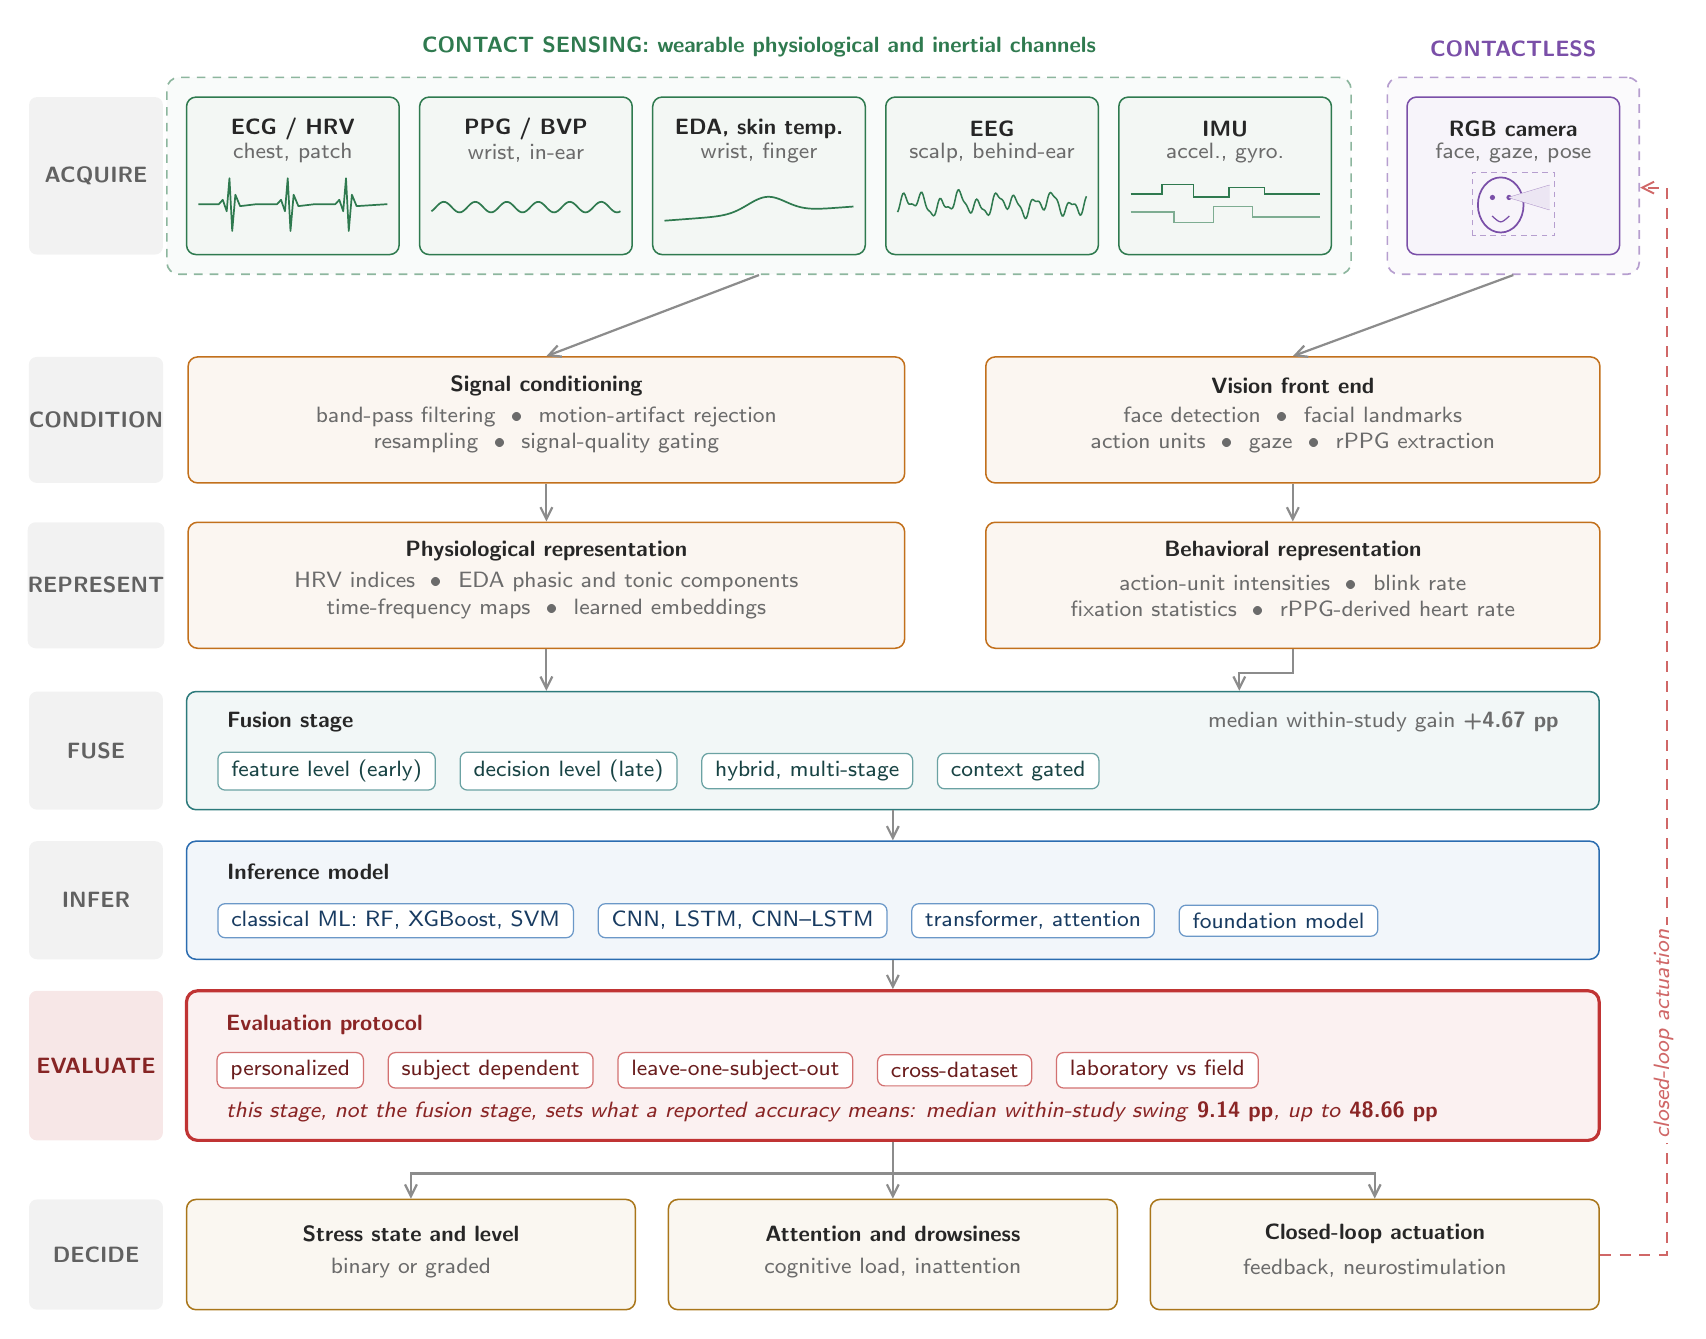
\begin{tikzpicture}[
  x=1mm, y=1mm,
  font=\sffamily,
  card/.style={rectangle, rounded corners=1.2mm, draw=#1, fill=#1!6,
               line width=0.55pt, align=center, inner sep=0pt},
  stage/.style={rectangle, rounded corners=1mm, fill=black!5, draw=none,
                inner sep=0pt, minimum width=17mm, align=center,
                font=\sffamily\bfseries\footnotesize, text=black!62},
  chip/.style={rectangle, rounded corners=0.9mm, draw=#1!70, fill=white,
               line width=0.45pt, inner xsep=1.7mm, inner ysep=1.0mm,
               font=\sffamily\footnotesize, text=#1!55!black},
  flow/.style={-{Straight Barb[length=1.5mm, width=1.5mm]},
               line width=0.8pt, draw=black!45},
  loop/.style={-{Straight Barb[length=1.5mm, width=1.5mm]},
               line width=0.7pt, draw=RED!75, dash pattern=on 1.4mm off 1.1mm},
  ttl/.style={font=\sffamily\bfseries\footnotesize, text=black!85},
  sub/.style={font=\sffamily\footnotesize, text=black!58},
]

\definecolor{GRN}{HTML}{2F7A4F}
\definecolor{PUR}{HTML}{7A4FA8}
\definecolor{ORG}{HTML}{C2701C}
\definecolor{BLU}{HTML}{2B6CB0}
\definecolor{RED}{HTML}{C03434}
\definecolor{TEA}{HTML}{2C7A7B}
\definecolor{GLD}{HTML}{A9761A}

%% ---------- geometry ----------
\def\SW{27}   % sensor card width
\def\SH{20}   % sensor card height
\def\GAP{2.6} % gap between sensor cards
\def\LX{-25}  % stage label column x

% mini waveform helper: #1 colour, #2 anchor node, #3 y-offset, #4 coords
\newcommand{\wave}[3]{\draw[line width=0.55pt, draw=#1, line cap=round] #2 #3;}

%% ================= STAGE 1 : ACQUISITION =================
\node[card=GRN, minimum width=\SW mm, minimum height=\SH mm] (s1) at (0,0) {};
\node[card=GRN, minimum width=\SW mm, minimum height=\SH mm] (s2) at (\SW+\GAP,0) {};
\node[card=GRN, minimum width=\SW mm, minimum height=\SH mm] (s3) at (2*\SW+2*\GAP,0) {};
\node[card=GRN, minimum width=\SW mm, minimum height=\SH mm] (s4) at (3*\SW+3*\GAP,0) {};
\node[card=GRN, minimum width=\SW mm, minimum height=\SH mm] (s5) at (4*\SW+4*\GAP,0) {};
\node[card=PUR, minimum width=\SW mm, minimum height=\SH mm] (s6)
      at (5*\SW+5*\GAP+7,0) {};

\foreach \n/\t/\l in {s1/{ECG / HRV}/{chest, patch},
                      s2/{PPG / BVP}/{wrist, in-ear},
                      s3/{EDA, skin temp.}/{wrist, finger},
                      s4/{EEG}/{scalp, behind-ear},
                      s5/{IMU}/{accel., gyro.},
                      s6/{RGB camera}/{face, gaze, pose}} {
  \node[ttl] at ([yshift=6.0mm]\n.center) {\t};
  \node[sub] at ([yshift=2.9mm]\n.center) {\l};
}

% --- signal glyphs ---
\begin{scope}[shift={([yshift=-3.6mm]s1.center)}]   % ECG
  \draw[line width=0.62pt, draw=GRN, line join=round]
    (-12,0) -- (-9.4,0) -- (-8.9,0.55) -- (-8.4,-0.9) -- (-8.05,3.3)
    -- (-7.7,-3.4) -- (-7.3,1.2) -- (-6.7,-0.25) -- (-4.6,0)
    -- (-2.0,0) -- (-1.5,0.55) -- (-1.0,-0.9) -- (-0.65,3.3)
    -- (-0.3,-3.4) -- (0.1,1.2) -- (0.7,-0.25) -- (2.8,0)
    -- (5.4,0) -- (5.9,0.55) -- (6.4,-0.9) -- (6.75,3.3)
    -- (7.1,-3.4) -- (7.5,1.2) -- (8.1,-0.25) -- (12,0);
\end{scope}
\begin{scope}[shift={([yshift=-3.6mm]s2.center)}]   % PPG
  \draw[line width=0.62pt, draw=GRN, smooth]
    plot[domain=-12:12, samples=110]
    (\x, {1.05*sin((\x+12)*45)^2 + 0.42*sin((\x+12)*90) - 0.9});
\end{scope}
\begin{scope}[shift={([yshift=-3.6mm]s3.center)}]   % EDA
  \draw[line width=0.62pt, draw=GRN, smooth]
    plot[domain=-12:12, samples=80]
    (\x, {-2.1 + 0.075*(\x+12) + 2.05*exp(-((\x-1)/3.4)^2)});
\end{scope}
\begin{scope}[shift={([yshift=-3.6mm]s4.center)}]   % EEG
  \draw[line width=0.55pt, draw=GRN, smooth]
    plot[domain=-12:12, samples=180]
    (\x, {0.95*sin(\x*152) + 0.62*sin(\x*63) + 0.34*sin(\x*311)});
\end{scope}
\begin{scope}[shift={([yshift=-3.6mm]s5.center)}]   % IMU
  \draw[line width=0.55pt, draw=GRN]
    (-12,1.3) -- (-8,1.3) -- (-8,2.5) -- (-4,2.5) -- (-4,0.9) -- (0.5,0.9)
    -- (0.5,2.1) -- (5,2.1) -- (5,1.3) -- (12,1.3);
  \draw[line width=0.55pt, draw=GRN!62]
    (-12,-1.0) -- (-6.5,-1.0) -- (-6.5,-2.3) -- (-1.5,-2.3) -- (-1.5,-0.3)
    -- (3.5,-0.3) -- (3.5,-1.6) -- (12,-1.6);
\end{scope}
\begin{scope}[shift={([yshift=-3.7mm]s6.center)}]   % camera: face + gaze cone
  \draw[line width=0.5pt, draw=PUR!55, dash pattern=on 0.7mm off 0.6mm]
        (-5.2,-3.9) rectangle (5.2,4.1);
  \draw[line width=0.62pt, draw=PUR] (-1.6,0) ellipse [x radius=2.9, y radius=3.5];
  \fill[PUR] (-2.65,0.95) circle (0.33);
  \fill[PUR] (-0.55,0.95) circle (0.33);
  \draw[line width=0.45pt, draw=PUR] (-2.7,-1.4) .. controls (-1.6,-2.4) .. (-0.5,-1.4);
  \draw[line width=0.4pt, draw=PUR!55] (-0.55,0.95) -- (4.6,2.5);
  \draw[line width=0.4pt, draw=PUR!55] (-0.55,0.95) -- (4.6,-0.6);
  \fill[PUR!14] (-0.55,0.95) -- (4.6,2.5) -- (4.6,-0.6) -- cycle;
\end{scope}

% group frames
\begin{scope}[on background layer]
  \node[draw=GRN!55, dash pattern=on 1.1mm off 0.9mm, rounded corners=1.5mm,
        line width=0.6pt, fill=GRN!3, fit=(s1)(s5), inner sep=2.4mm] (wgrp) {};
  \node[draw=PUR!55, dash pattern=on 1.1mm off 0.9mm, rounded corners=1.5mm,
        line width=0.6pt, fill=PUR!3, fit=(s6), inner sep=2.4mm] (vgrp) {};
\end{scope}
\node[font=\sffamily\bfseries\footnotesize, text=GRN, above=1.3mm of wgrp.north]
      {CONTACT SENSING: wearable physiological and inertial channels};
\node[font=\sffamily\bfseries\footnotesize, text=PUR, above=1.3mm of vgrp.north]
      {CONTACTLESS};

%% ================= STAGE 2 : CONDITIONING =================
\def\CW{91}
\node[card=ORG, minimum width=\CW mm, minimum height=16mm] (c1) at (32.2,-31) {};
\node[card=ORG, minimum width=78mm, minimum height=16mm] (c2) at (127,-31) {};
\node[ttl] at ([yshift=4.3mm]c1.center) {Signal conditioning};
\node[sub, align=center] at ([yshift=-1.3mm]c1.center)
      {band-pass filtering \ \textbullet\ \ motion-artifact rejection\\
       resampling \ \textbullet\ \ signal-quality gating};
\node[ttl] at ([yshift=4.3mm]c2.center) {Vision front end};
\node[sub, align=center] at ([yshift=-1.3mm]c2.center)
      {face detection \ \textbullet\ \ facial landmarks\\
       action units \ \textbullet\ \ gaze \ \textbullet\ \ rPPG extraction};

%% ================= STAGE 3 : REPRESENTATION =================
\node[card=ORG, minimum width=\CW mm, minimum height=16mm] (r1) at (32.2,-52) {};
\node[card=ORG, minimum width=78mm, minimum height=16mm] (r2) at (127,-52) {};
\node[ttl] at ([yshift=4.3mm]r1.center) {Physiological representation};
\node[sub, align=center] at ([yshift=-1.3mm]r1.center)
      {HRV indices \ \textbullet\ \ EDA phasic and tonic components\\
       time-frequency maps \ \textbullet\ \ learned embeddings};
\node[ttl] at ([yshift=4.3mm]r2.center) {Behavioral representation};
\node[sub, align=center] at ([yshift=-1.3mm]r2.center)
      {action-unit intensities \ \textbullet\ \ blink rate\\
       fixation statistics \ \textbullet\ \ rPPG-derived heart rate};

%% ================= STAGE 4 : FUSION =================
\node[card=TEA, minimum width=179.4mm, minimum height=15mm] (fu) at (76.2,-73) {};
\node[ttl, anchor=west] at ([xshift=4mm,yshift=3.6mm]fu.west) {Fusion stage};
\node[chip=TEA, anchor=west] (f1) at ([xshift=4mm,yshift=-2.6mm]fu.west)
      {feature level (early)};
\node[chip=TEA, right=3mm of f1] (f2) {decision level (late)};
\node[chip=TEA, right=3mm of f2] (f3) {hybrid, multi-stage};
\node[chip=TEA, right=3mm of f3] (f4) {context gated};
\node[sub, anchor=east] at ([xshift=-4mm,yshift=3.6mm]fu.east)
      {median within-study gain \textbf{+4.67 pp}};

%% ================= STAGE 5 : INFERENCE =================
\node[card=BLU, minimum width=179.4mm, minimum height=15mm] (inf) at (76.2,-92) {};
\node[ttl, anchor=west] at ([xshift=4mm,yshift=3.6mm]inf.west) {Inference model};
\node[chip=BLU, anchor=west] (i1) at ([xshift=4mm,yshift=-2.6mm]inf.west)
      {classical ML: RF, XGBoost, SVM};
\node[chip=BLU, right=3mm of i1] (i2) {CNN, LSTM, CNN--LSTM};
\node[chip=BLU, right=3mm of i2] (i3) {transformer, attention};
\node[chip=BLU, right=3mm of i3] (i4) {foundation model};

%% ================= STAGE 6 : EVALUATION (focus) =================
\node[rectangle, rounded corners=1.4mm, draw=RED, fill=RED!7, line width=1.15pt,
      minimum width=179.4mm, minimum height=19mm, inner sep=0pt] (ev) at (76.2,-113) {};
\node[ttl, anchor=west, text=RED!72!black]
      at ([xshift=4mm,yshift=5.2mm]ev.west) {Evaluation protocol};
\node[chip=RED, anchor=west] (e1) at ([xshift=4mm,yshift=-0.6mm]ev.west) {personalized};
\node[chip=RED, right=3mm of e1] (e2) {subject dependent};
\node[chip=RED, right=3mm of e2] (e3) {leave-one-subject-out};
\node[chip=RED, right=3mm of e3] (e4) {cross-dataset};
\node[chip=RED, right=3mm of e4] (e5) {laboratory vs field};
\node[font=\sffamily\itshape\footnotesize, text=RED!72!black, anchor=west]
      at ([xshift=4mm,yshift=-5.9mm]ev.west)
      {this stage, not the fusion stage, sets what a reported accuracy means:
       median within-study swing \textbf{9.14 pp}, up to \textbf{48.66 pp}};

%% ================= STAGE 7 : OUTPUT =================
\node[card=GLD, minimum width=57mm, minimum height=14mm] (o1) at (15,-137) {};
\node[card=GLD, minimum width=57mm, minimum height=14mm] (o2) at (76.2,-137) {};
\node[card=GLD, minimum width=57mm, minimum height=14mm] (o3) at (137.4,-137) {};
\node[ttl] at ([yshift=2.6mm]o1.center) {Stress state and level};
\node[sub] at ([yshift=-1.7mm]o1.center) {binary or graded};
\node[ttl] at ([yshift=2.6mm]o2.center) {Attention and drowsiness};
\node[sub] at ([yshift=-1.7mm]o2.center) {cognitive load, inattention};
\node[ttl] at ([yshift=2.6mm]o3.center) {Closed-loop actuation};
\node[sub] at ([yshift=-1.7mm]o3.center) {feedback, neurostimulation};

%% ================= stage labels =================
\node[stage, minimum height=\SH mm]  at (\LX, 0)    {ACQUIRE};
\node[stage, minimum height=16mm]    at (\LX,-31)   {CONDITION};
\node[stage, minimum height=16mm]    at (\LX,-52)   {REPRESENT};
\node[stage, minimum height=15mm]    at (\LX,-73)   {FUSE};
\node[stage, minimum height=15mm]    at (\LX,-92)   {INFER};
\node[stage, minimum height=19mm, fill=RED!12, text=RED!70!black] at (\LX,-113) {EVALUATE};
\node[stage, minimum height=14mm]    at (\LX,-137)  {DECIDE};

%% ================= flow arrows =================
\draw[flow] (wgrp.south) -- (c1.north);
\draw[flow] (vgrp.south) -- (c2.north);
\draw[flow] (c1) -- (r1);
\draw[flow] (c2) -- (r2);
\draw[flow] (r1.south) -- ++(0,-3) -| ([xshift=-44mm]fu.north);
\draw[flow] (r2.south) -- ++(0,-3) -| ([xshift=44mm]fu.north);
\draw[flow] (fu) -- (inf);
\draw[flow] (inf) -- (ev);
\draw[flow] (ev.south) -- ++(0,-4) -| (o1.north);
\draw[flow] (ev.south) -- ++(0,-4) -| (o2.north);
\draw[flow] (ev.south) -- ++(0,-4) -| (o3.north);
\draw[loop] (o3.east) -- ++(8.5,0) |- ([yshift=-1.5mm]vgrp.east);
\node[font=\sffamily\itshape\footnotesize, text=RED!75, anchor=south, align=center,
      fill=white, inner sep=0.6mm, rotate=90]
      at ([xshift=10mm,yshift=28mm]o3.east) {closed-loop actuation};
\end{tikzpicture}
}
\caption{Seven-stage processing chain shared by the wearable and camera-based stress and
attention monitoring systems reviewed here, with a representative trace drawn inside each
acquisition card. Contact channels (green) and the contactless camera channel (purple) are
conditioned and represented separately before being combined at a feature, decision, hybrid
or context-gated fusion stage and passed to an inference model. The evaluation protocol is
drawn as a stage of equal standing, and highlighted, because it is the stage that determines
what a reported accuracy means: the median within-study swing attributable to it is 9.14
percentage points against 4.67 for the fusion stage. The dashed return path denotes
closed-loop actuation, in which a decision drives stimulation or feedback that the sensors
then observe.}
\label{fig:block}
\end{figure}

\subsection{Limitations of Unimodal Approaches and the Case for Integration}
Each modality fails in characteristic ways. Wearable signals are corrupted by motion
artifacts and variable skin contact, and physiological arousal caused by exertion is not
separable from arousal caused by stress without contextual information \cite{r19,r79}.
Camera-based systems depend on illumination, an unoccluded face and a favorable viewing
angle, and observe only the externally expressed surface of an internal state.

The standard argument is that these failure modes are complementary, so fusing the channels
should be more than additive. The argument is plausible, and several studies do report gains.
What is rarely examined is the magnitude of that gain once it is measured properly. Almost
all quantitative support for fusion in this literature is assembled by comparing the accuracy
reported by a multimodal study against the accuracy reported by a different unimodal study.
Those two numbers differ in cohort, stressor protocol, label source, class definition,
preprocessing and, critically, validation scheme. A between-study difference therefore
estimates the sum of all of these, not the effect of fusion. This review is built on the
observation that a much cleaner estimate is available and has not been systematically
exploited: within a single study, a single team frequently reports a unimodal baseline and a
fused model under an identical protocol, and separately reports the same model under two
different evaluation regimes. These within-study contrasts identify the fusion effect and the
evaluation effect on the same scale, and permit them to be compared directly.

\subsection{Research Questions and Objectives}
Prior reviews of wearable stress monitoring have documented that generalization is weak
\cite{r118}, and prior reviews of affective computing survey physiological and vision-based
modalities largely in parallel. Neither has quantified how the benefit attributed to fusion
compares with the performance swing produced by evaluation design. This review addresses that
gap through three questions:

\textbf{RQ1:} When fusion gain is estimated only from within-study, protocol-matched
comparisons, how large is it? This matters because every deployment decision that favors a
second sensor over a single one is justified by an assumed magnitude, and that magnitude has
never been isolated from its confounds.

\textbf{RQ2:} How does that fusion gain compare with the within-study performance difference
attributable to evaluation choices, namely personalization, deployment setting, dataset and
task granularity? This matters because if the second effect dominates, the field's
optimization target is misplaced.

\textbf{RQ3:} Has the dominant benchmark saturated, and how completely is the evidence base
reported and independently verifiable? This matters because a saturated benchmark combined
with unreported protocols makes architectural progress unfalsifiable.

The review pursues five objectives:
\begin{itemize}[leftmargin=1.25em,itemsep=1pt,topsep=2pt]
\item \textbf{O1:} Assemble a topically screened corpus of 2022 to 2026 studies in which every
      bibliographic record is independently corroborated.
\item \textbf{O2:} Carry only corroborated outcome values into the synthesis and report the
      corroboration and reporting-recovery rates as evidence in their own right.
\item \textbf{O3:} Estimate the within-study fusion gain under matched protocols.
\item \textbf{O4:} Estimate the within-study evaluation-induced gap and compare the two on a
      common scale.
\item \textbf{O5:} Test benchmark saturation and derive a reporting specification for
      translational work.
\end{itemize}

Section~2 reviews unimodal and integrated work and the limits of prior surveys. Section~3
gives the review and verification methodology. Section~4 reports results against the
objectives. Section~5 synthesizes the trends. Sections~6 and~7 discuss and conclude.

\section{Overview of Related Works}

\subsection{Unimodal Wearable Sensor-Based Approaches}
Single-channel wearable sensing remains a strong baseline and, importantly for the argument
developed here, frequently matches multimodal systems on public benchmarks. EDA is the most
direct peripheral index of sympathetic arousal and has been used alone for binary stress
classification across four public corpora \cite{r52} and in privacy-preserving federated
settings \cite{r72}. HRV derived from ECG supports stress classification in factory workers
\cite{r5}, physicians \cite{r1} and office employees \cite{r61}, and ECG-derived multifractal
descriptors have been proposed specifically to separate cognitive stress from physical
activity \cite{r56}.

PPG has attracted the most recent methodological attention because it is the channel
available on consumer hardware. Lightweight architectures operating on blood volume pulse
alone now report $98.23\%$ accuracy with an AUC of $0.9953$ on WESAD \cite{r50} and $96.94\%$
under leave-one-subject-out (LOSO) validation \cite{r55}, while a separable-attention dilated
network evaluated under LOSO across two cohorts reports $92.25\%$ \cite{r47}. In-ear PPG
transformed into time-frequency images and classified with a vision transformer reaches
$97.78\%$ \cite{r43}. EEG offers the greatest neurophysiological specificity, and miniaturised
behind-the-ear devices with on-chip inference have made it more practical \cite{r31},
although headset intrusiveness still limits naturalistic use.

The essential observation is that these unimodal systems are not obviously worse than the
multimodal systems they are implicitly compared against. That observation is the starting
point for the present analysis.

\subsection{Unimodal Computer Vision-Based Approaches}
Camera-based affect and attention sensing rests on facial expression analysis, gaze and blink
dynamics, head pose and camera-derived physiological proxies. Facial action unit decomposition
supports inference of cognitive load and engagement, and gaze statistics such as fixation
duration and blink rate index attentional focus and fatigue.

Remote PPG is the most direct bridge between the two sensing families because it recovers a
cardiac signal without contact. A multi-task attentional convolutional network operating on
rPPG extracted from facial video reports $94.33\%$ accuracy for binary stress state and
$83.83\%$ for graded stress level \cite{r16}, a within-study contrast we return to in
Section~4.3. Camera-based systems nevertheless remain constrained by illumination, occlusion
and viewing angle, and observe behavior rather than autonomic state.

\subsection{Integrated Systems and the Limits of Prior Surveys}
Integration has progressed from simple concatenation of physiological and visual features
before a shared classifier, through decision-level combination of modality-specific
classifiers, to hybrid and context-gated schemes that adapt the fusion rule to sensing
conditions \cite{r58,r79}. Genuinely integrated wearable and camera systems exist: facial
features extracted from RGB video have been combined with wearable PPG and EDA for workplace
stress assessment \cite{r17}, and physiological wristband features have been combined with
facial action units and gaze in an office cohort \cite{r26}. Closed-loop designs that couple
PPG-based sensing to transcutaneous median nerve stimulation for acute stress mitigation
\cite{r38} and multimodal bioelectronic wristbands that add molecular biomarkers to
physiological channels \cite{r108} extend the same architecture towards therapeutic control.

Existing reviews, however, treat the two sensing families largely in parallel and synthesize
performance by pooling headline numbers. The most rigorous prior synthesis concluded that
most wearable stress models lack generalization \cite{r118}, a qualitative verdict that this
review converts into a quantitative one. No prior survey, to our knowledge, restricts its
quantitative synthesis to within-study contrasts, and none places the fusion effect and the
evaluation effect on a common scale. That is the gap addressed here.

\section{Methodology}

\subsection{Search Strategy and Corpus Construction}
The review covers peer-reviewed journal articles published between 1 January 2022 and
31 March 2026 that report quantitative detection or monitoring of stress, attention,
drowsiness or cognitive load from wearable physiological sensing, camera-based sensing, or
their combination. The source corpus comprised 117 numbered bibliographic records assembled
from IEEE Xplore, ScienceDirect, MDPI, PLOS, SpringerLink, JMIR and BMC across the wearable
sensing, affective state monitoring and machine learning literatures. One record was a
duplicate citation of a study already present, leaving 116 unique records for screening.

Because the analytic claims of this review depend on the integrity of the underlying records,
corpus composition is reported by publisher of record rather than by an unverifiable count of
raw database hits. Table~\ref{tab:t1} gives the screening yield for each publisher. IEEE
titles dominate both the screened pool and the included set, reflecting the concentration of
wearable sensing methodology in IEEE sensor, biomedical and affective computing journals,
while the PLOS records show the lowest inclusion yield because that portion of the pool is
weighted towards clinical and device-validation work outside the present scope.

\begin{table}[H]
\centering
\caption{Composition of the screened corpus and inclusion yield by publisher of record.
Inclusion yield is the proportion of screened records from that publisher that met all
eligibility criteria.}
\label{tab:t1}
\small
\resizebox{\textwidth}{!}{\begin{tabular}{L{3.7cm} C{2.3cm} C{2.3cm} C{2.3cm} C{2.4cm}}
\toprule
\textbf{Publisher of record} & \textbf{Records screened} & \textbf{Studies included} & \textbf{Records excluded} & \textbf{Inclusion yield (\%)} \\
\midrule
IEEE & 30 & 27 & 3 & 90.0 \\
PLOS & 22 & 6 & 16 & 27.3 \\
Elsevier & 21 & 8 & 13 & 38.1 \\
Springer Nature & 16 & 4 & 12 & 25.0 \\
MDPI & 11 & 10 & 1 & 90.9 \\
JMIR & 7 & 2 & 5 & 28.6 \\
Springer & 3 & 2 & 1 & 66.7 \\
BMC & 2 & 1 & 1 & 50.0 \\
medRxiv & 1 & 0 & 1 & 0.0 \\
Research Square & 1 & 0 & 1 & 0.0 \\
ACM & 1 & 0 & 1 & 0.0 \\
RSC & 1 & 0 & 1 & 0.0 \\
\midrule
\textbf{Total} & \textbf{116} & \textbf{60} & \textbf{56} & \textbf{51.7} \\
\bottomrule
\end{tabular}}
\end{table}

\subsection{Inclusion and Exclusion Criteria}
Eligibility was assessed against the pre-specified criteria in Table~\ref{tab:t2}. Two
criteria differ from common practice in this literature and account for most exclusions.
First, the outcome criterion is strict: a study qualifies only if it reports a psychological
stress, attention, drowsiness or cognitive-load outcome. Wearable studies whose outcome is
cardiac arrhythmia, sleep staging, seizure detection, glucose, physical fatigue, human
activity recognition or materials characterisation were excluded even when they are
frequently cited in stress-monitoring reviews, because pooling them inflates apparent
coverage without contributing evidence about the states of interest. Second, independent
corroboration of the bibliographic record was itself a requirement rather than a courtesy.

\begin{table}[H]
\centering
\caption{Eligibility criteria and the number of records excluded under each. Exclusion
reasons are mutually exclusive and were applied in the order listed.}
\label{tab:t2}
\small
\resizebox{\textwidth}{!}{%
\begin{tabular}{L{2.4cm} L{5.7cm} L{6.3cm} C{1.6cm}}
\toprule
\textbf{Domain} & \textbf{Included} & \textbf{Excluded} & \textbf{Records excluded} \\
\midrule
Publication window & Published January 2022 to March 2026. & Published before January 2022.
  & 2 \\
Publication type & Peer-reviewed journal article. & Preprints, conference papers, book
  chapters, editorials. & 3 \\
Outcome & Psychological stress, attention, inattention, drowsiness, cognitive load or mental
  workload. & Any other physiological or clinical outcome, including arrhythmia, sleep
  staging, seizures, glucose, physical fatigue and activity recognition. & 41 \\
Study type & Empirical study reporting a quantitative evaluation of a detection or
  monitoring model. & Study protocols, narrative reviews, technology-acceptance studies and
  intervention trials without a detection model. & 10 \\
Technology & Wearable physiological or inertial sensing, camera-based sensing, or their
  fusion, with an ML or DL model. & Purely theoretical work with no applied sensing
  component. & 0 \\
Verifiability & Bibliographic record independently corroborated against the publisher or
  indexed record. & Record that could not be corroborated. & 0 \\
\midrule
\multicolumn{3}{l}{\textbf{Total excluded}} & \textbf{56} \\
\multicolumn{3}{l}{\textbf{Total included}} & \textbf{60} \\
\bottomrule
\end{tabular}}
\end{table}

\subsection{Screening, Selection and Verification}
Screening followed PRISMA and is summarized in Figure~\ref{fig:prisma}. Of 116 unique records,
56 were excluded at eligibility appraisal, 41 of them because the reported outcome fell
outside the stress, attention and cognitive-load scope, 10 because no quantitative model
evaluation was reported, 3 because the record was a preprint or conference paper and 2
because it fell outside the publication window. Sixty studies met all criteria.

Verification was then applied to all 60 included studies. For each, the title, authors,
journal, year, volume, pagination and DOI were checked against the publisher or indexed
record, and the reported headline outcome was sought in the same source. A value was carried
into the quantitative synthesis only where it could be recovered from the openly retrievable
record; values that could not be recovered were left coded as not recovered rather than
imputed, and no value was taken on the authority of a secondary citation. Twenty-eight of the
60 studies yielded a corroborated headline outcome, contributing 34 outcome records, 4
within-study fusion contrasts and 10 within-study evaluation contrasts. The remaining 32
studies are retained in the narrative synthesis, where their design and findings are
described, but contribute no numbers.

\begin{figure}[H]
\centering
\resizebox{0.95\textwidth}{!}{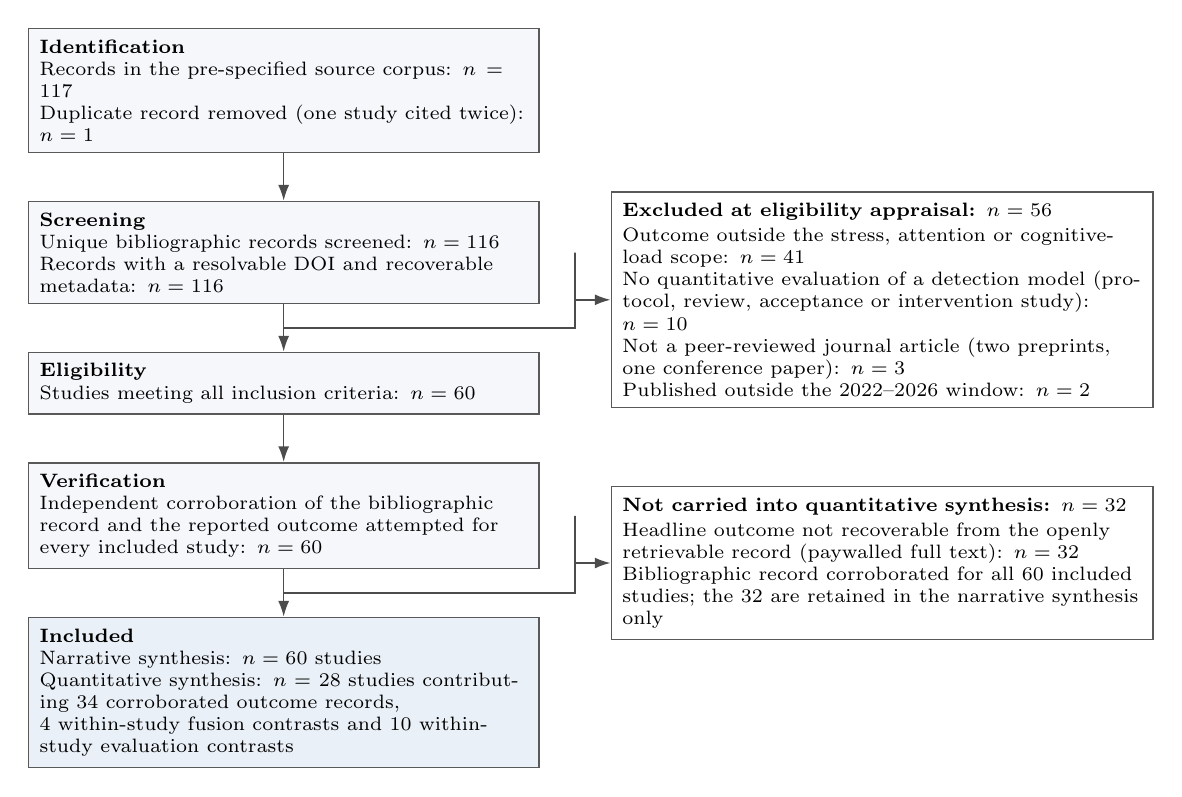
\begin{tikzpicture}[node distance=5mm]

\node[pr] (r1) {\textbf{Identification}\\
  Records in the pre-specified source corpus: $n=117$\\
  Duplicate record removed (one study cited twice): $n=1$};

\node[pr,below=6mm of r1] (r2) {\textbf{Screening}\\
  Unique bibliographic records screened: $n=116$\\
  Records with a resolvable DOI and recoverable metadata: $n=116$};

\node[prx,anchor=west] (x1) at ($(r2.east)+(9mm,-6mm)$) {\textbf{Excluded at eligibility appraisal: $n=56$}\\[1pt]
  Outcome outside the stress, attention or cognitive-load scope: $n=41$\\
  No quantitative evaluation of a detection model
  (protocol, review, acceptance or intervention study): $n=10$\\
  Not a peer-reviewed journal article (two preprints, one conference paper): $n=3$\\
  Published outside the 2022--2026 window: $n=2$};

\node[pr,below=6mm of r2] (r3) {\textbf{Eligibility}\\
  Studies meeting all inclusion criteria: $n=60$};

\node[pr,below=6mm of r3] (r4) {\textbf{Verification}\\
  Independent corroboration of the bibliographic record and the
  reported outcome attempted for every included study: $n=60$};

\node[prx,anchor=west] (x2) at ($(r4.east)+(9mm,-6mm)$) {\textbf{Not carried into quantitative synthesis: $n=32$}\\[1pt]
  Headline outcome not recoverable from the openly retrievable
  record (paywalled full text): $n=32$\\
  Bibliographic record corroborated for all 60 included studies; the
  32 are retained in the narrative synthesis only};

\node[pr,below=6mm of r4,fill=acc!10] (r5) {\textbf{Included}\\
  Narrative synthesis: $n=60$ studies\\
  Quantitative synthesis: $n=28$ studies contributing 34 corroborated
  outcome records,\\ 4 within-study fusion contrasts and 10 within-study
  evaluation contrasts};

\draw[ar] (r1) -- (r2);
\draw[ar] (r2) -- (r3);
\draw[ar] (r3) -- (r4);
\draw[ar] (r4) -- (r5);
\draw[ar] ($(r2.south)!0.5!(r3.north)$) -| ($(r2.east)+(4.5mm,0)$) |- (x1.west);
\draw[ar] ($(r4.south)!0.5!(r5.north)$) -| ($(r4.east)+(4.5mm,0)$) |- (x2.west);
\end{tikzpicture}
}
\caption{PRISMA flow of record identification, screening, eligibility appraisal, independent
verification and inclusion. The verification stage is additional to the standard PRISMA
template and is reported because it determines which studies contribute quantitative
evidence.}
\label{fig:prisma}
\end{figure}

Figure~\ref{fig:corpus} characterizes the included corpus. Figure~\ref{fig:corpus}(a) shows
the number of included studies per publication year, decomposed by application area, and
Figure~\ref{fig:corpus}(b) shows the aggregate distribution across application areas. Output
grew from 6 studies in 2022 to 17 in 2025, with 9 in the partial 2026 window. Laboratory
studies dominate at 19 of 60 (32\%), and a further 12 (20\%) are benchmark-only studies that
report no new data collection at all. Together these account for just over half the corpus,
whereas free-living daily-life deployments account for 9 (15\%) and the high-consequence
driving and aviation settings that most motivate the field account for 4 (7\%) combined. The
evidence base is therefore concentrated precisely where evaluation conditions are most
favorable and least representative of deployment.

\begin{figure}[H]
\centering
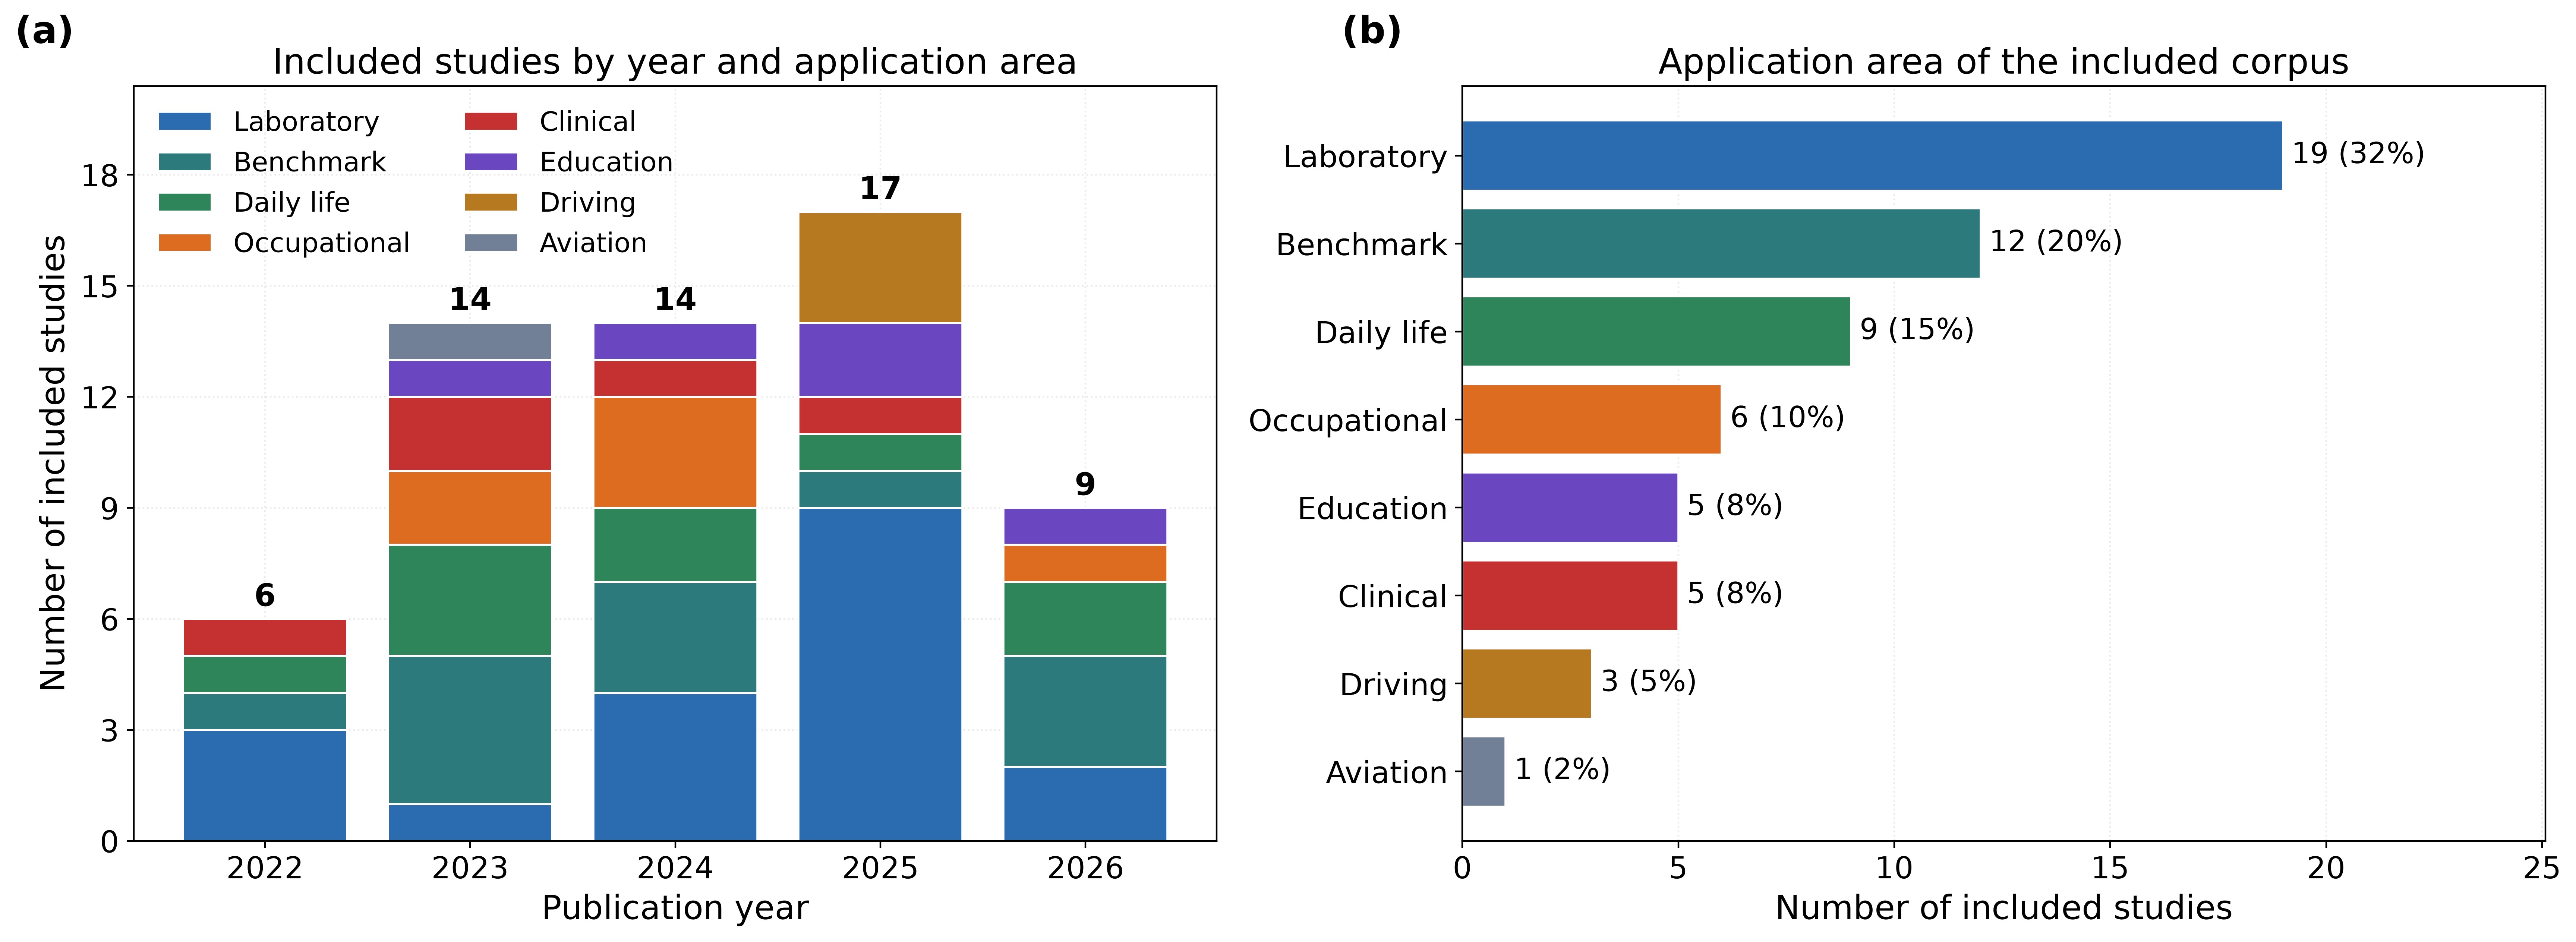
\includegraphics[width=0.99\textwidth]{fig3_corpus.png}
\caption{Composition of the included corpus. Figure~\ref{fig:corpus}(a) shows the number of
included studies per publication year, with each bar decomposed by application area and the
annual total printed above the bar. Figure~\ref{fig:corpus}(b) shows the total number of
included studies in each application area with the corresponding percentage of the corpus.}
\label{fig:corpus}
\end{figure}

Figure~\ref{fig:screen} summarizes the screening outcome. Figure~\ref{fig:screen}(a) shows the
number of records excluded under each eligibility criterion, and Figure~\ref{fig:screen}(b)
shows the publisher of record for the included studies. Out-of-scope outcomes account for 41
of 56 exclusions (73\%), which quantifies how much of the material customarily cited in this
area does not in fact report a stress or attention outcome.

\begin{figure}[H]
\centering
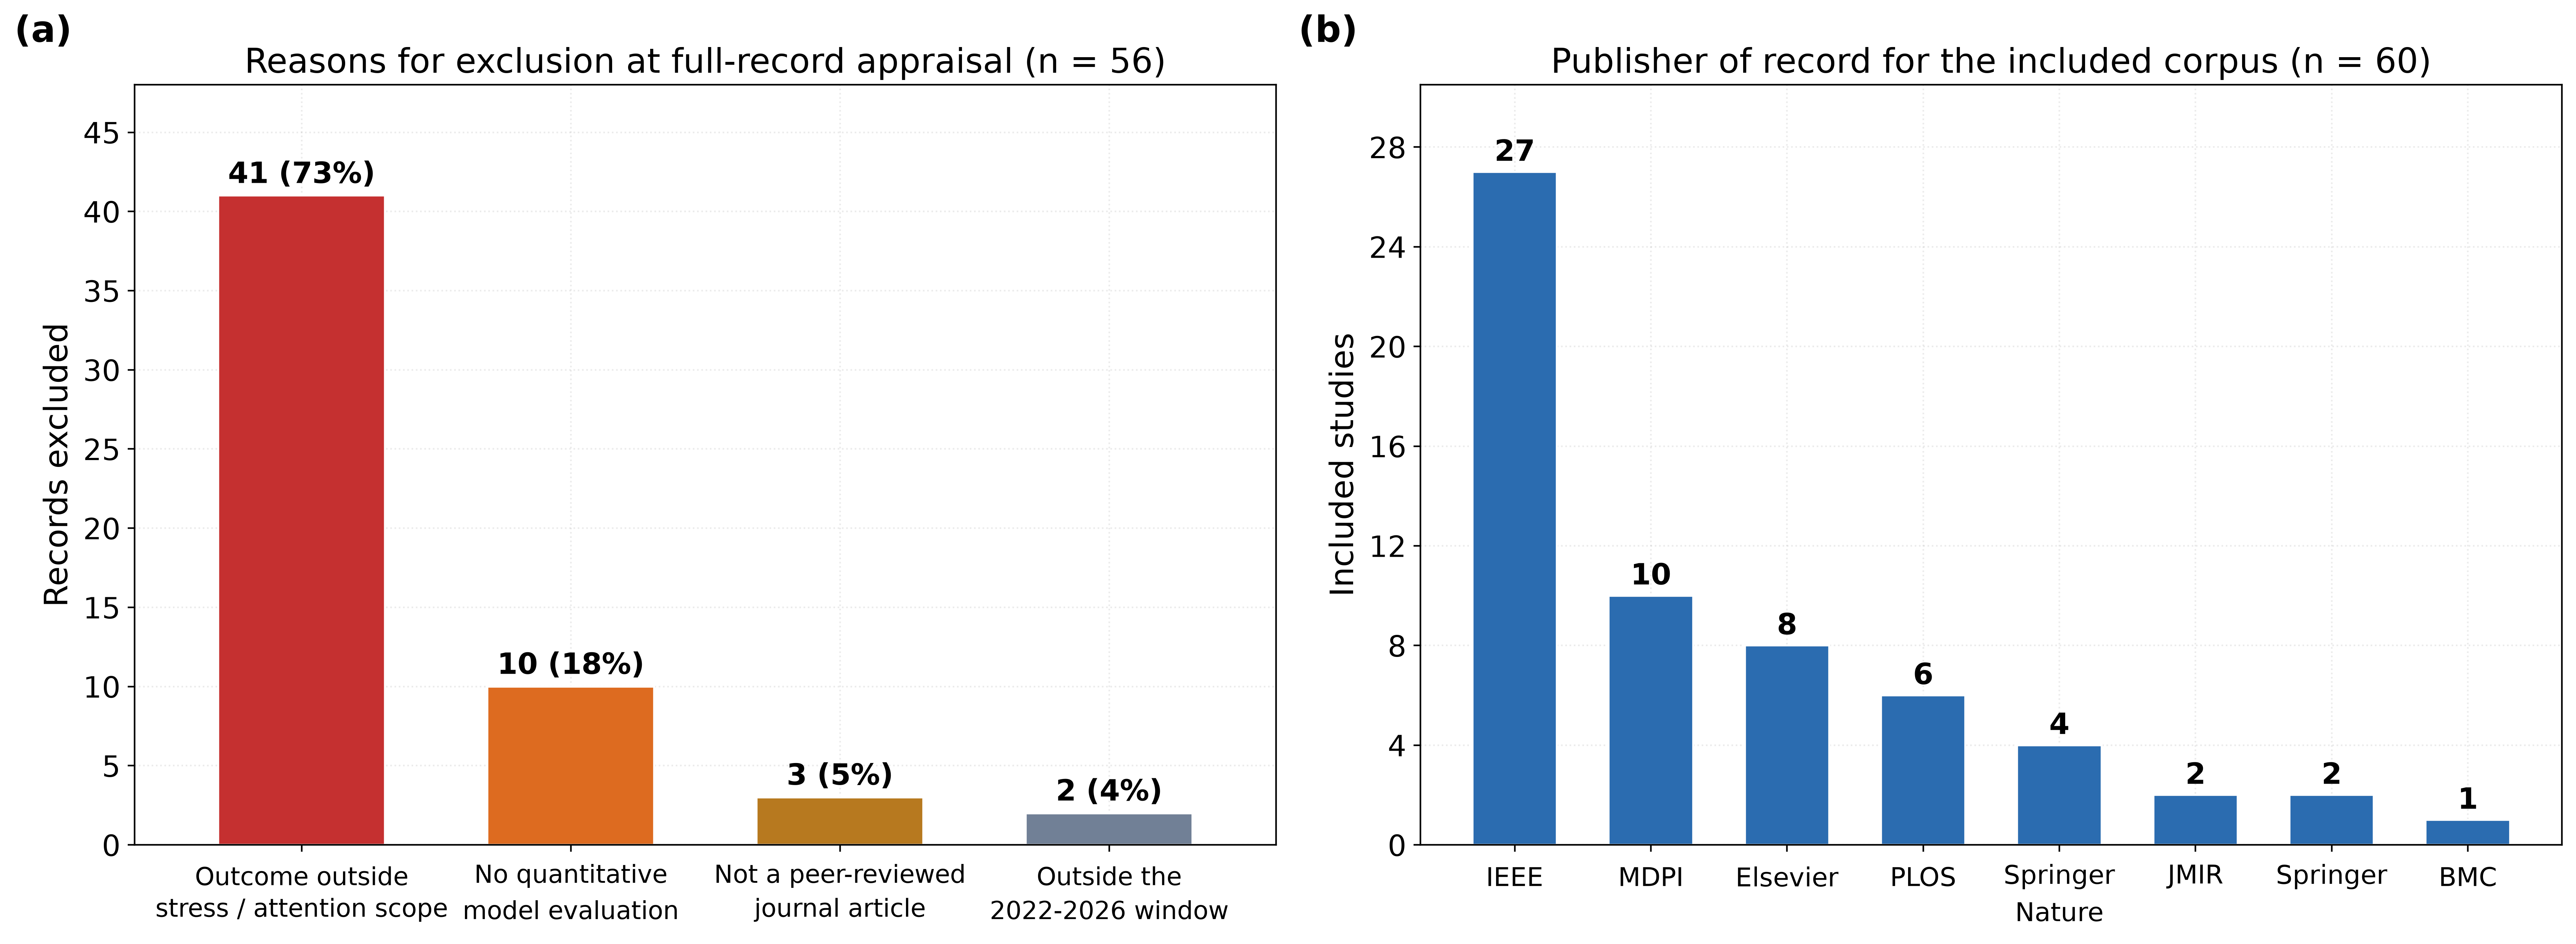
\includegraphics[width=0.99\textwidth]{fig4_screening.png}
\caption{Screening outcome and corpus provenance. Figure~\ref{fig:screen}(a) shows the number
of records excluded under each eligibility criterion, with the percentage of all exclusions
annotated. Figure~\ref{fig:screen}(b) shows the publisher of record for the 60 included
studies.}
\label{fig:screen}
\end{figure}

\subsection{Reporting Appraisal}
In place of a generic quality checklist, each included study was appraised on whether five
items material to interpreting a reported result could actually be recovered: the headline
performance metric, the size of the evaluation cohort, the validation protocol, whether a
public benchmark was used, and whether any variance or confidence interval accompanied the
point estimate. These items were chosen because each is necessary to decide whether a
reported number transfers. Results are given in Table~\ref{tab:t3} and analyzed in
Section~4.4.

\begin{table}[H]
\centering
\caption{Recovery of reporting items across all 60 included studies. An item is counted as
recovered only where it was explicitly obtained from the openly retrievable record during
verification. Rates therefore bound, from below, how completely this evidence base can be
interpreted by a reader without subscription access.}
\label{tab:t3}
\small
\resizebox{\textwidth}{!}{\begin{tabular}{L{5.4cm} C{2.6cm} C{2.6cm} C{3.1cm}}
\toprule
\textbf{Reporting item} & \textbf{Recovered ($k$)} & \textbf{Not recovered} & \textbf{Recovery rate (\%)} \\
\midrule
Headline metric & 28 & 32 & 46.7 \\
Evaluation cohort size & 18 & 42 & 30.0 \\
Validation protocol & 8 & 52 & 13.3 \\
Public benchmark used & 14 & 46 & 23.3 \\
Variance or CI reported & 3 & 57 & 5.0 \\
\bottomrule
\end{tabular}}
\end{table}

\subsection{Synthesis Strategy}
Two estimands are defined. The \textbf{fusion gain} is the difference, within one study,
between the best single-modality result and the multimodal result obtained on the same
cohort, with the same pipeline and under the same validation protocol. The
\textbf{evaluation-induced gap} is the difference, within one study, between the most
favorable and the most realistic evaluation condition reported for the same model, where
the varied factor is personalization, deployment setting, dataset or task granularity.

Restricting both estimands to within-study contrasts removes the between-study confounds of
cohort, stressor, labeling and preprocessing, at the cost of a small number of eligible
contrasts. Given that $k$, effect sizes are summarized by the median and full range rather
than by a pooled random-effects estimate, and no significance testing is performed; the
comparison of interest is the relative magnitude of two medians, not a hypothesis test.
Accuracy and AUROC differences are both expressed in percentage points (pp) and are reported
separately by metric in the tables so that no cross-metric arithmetic is implied.

\section{Results}

\subsection{The Corroborated Evidence Base}
Table~\ref{tab:t4} lists every outcome record carried into the synthesis, with its sensing
configuration, evaluation data, cohort size, validation protocol, metric and value. Across
the 29 accuracy records the median is $93.00\%$ with an interquartile range of
$87.37$ to $96.09\%$. Two features of the table are more informative than that central
tendency. First, the protocol column is dominated by \textit{Not reported}: only 8 of the 60
included studies state a validation protocol recoverably, so for most records it cannot be
determined whether the reported number reflects subject-dependent or subject-independent
performance. Second, the highest values in the table belong to unimodal systems. Blood volume
pulse alone reaches $98.23\%$ on WESAD \cite{r50}, and in-ear PPG alone reaches $97.78\%$
\cite{r43}, both above every multimodal record in the table. This is already inconsistent
with a strong reading of the fusion hypothesis.

\begin{table}[H]
\centering
\caption{Corroborated outcome records contributing to the quantitative synthesis. Every value
was recovered from the publisher or indexed record; no value is taken from a secondary
citation. LOSO denotes leave-one-subject-out validation and NR denotes a cohort size or
protocol that could not be recovered.}
\label{tab:t4}
\scriptsize
\resizebox{\textwidth}{!}{\begin{tabular}{L{2.8cm} C{0.7cm} L{3.2cm} L{2.45cm} C{0.7cm} L{1.8cm} C{0.9cm} C{1.1cm}}
\toprule
\textbf{Study} & \textbf{Year} & \textbf{Sensing configuration} & \textbf{Evaluation data} & \textbf{$n$} & \textbf{Protocol} & \textbf{Metric} & \textbf{Value (\%)} \\
\midrule
Abdul Kader et al. \cite{r75} & 2024 & EEG+GSR & In-house & 20 & Not reported & Accuracy & 84.60 \\
Ali et al. (ReTeNet) \cite{r50} & 2025 & BVP & WESAD & 15 & Not reported & Accuracy & 98.23 \\
Ali et al. (SADDNet) \cite{r47} & 2026 & PPG & CATSA+WESAD & 50 & LOSO & Accuracy & 92.25 \\
Ali et al. (TEANet) \cite{r55} & 2026 & BVP & WESAD & 15 & LOSO & Accuracy & 96.94 \\
Ali et al. (TEANet) \cite{r55} & 2026 & BVP & RUET-SPML & 19 & LOSO & Accuracy & 92.94 \\
Alsahreef et al. \cite{r1} & 2026 & HRV & PARFAIT & NR & Not reported & Accuracy & 98.10 \\
Awada et al. \cite{r26} & 2024 & EDA+BVP+TEMP+behav. & In-house (office) & NR & Not reported & Accuracy & 82.78 \\
Barki et al. \cite{r43} & 2025 & In-ear PPG & In-house & 15 & Not reported & Accuracy & 97.78 \\
Campanella et al. \cite{r12} & 2023 & PPG+EDA & In-house & 29 & Not reported & Accuracy & 90.00 \\
Chen \& Lee \cite{r74} & 2023 & ECG & In-house & NR & Not reported & Accuracy & 93.42 \\
Donati et al. \cite{r5} & 2023 & ECG & In-house (factory) & NR & Not reported & Accuracy & 88.40 \\
El Arwadi \& Abu Daher \cite{r21} & 2025 & ECG (HRV) & In-house & NR & LOSO & Accuracy & 90.80 \\
Fernandez et al. \cite{r30} & 2025 & EEG & In-house & NR & Subject indep. & Accuracy & 86.24 \\
Gedam et al. \cite{r99} & 2025 & ECG+GSR+TEMP & In-house & 200 & Not reported & Accuracy & 96.17 \\
Hongn et al. \cite{r19} & 2025 & EDA+BVP+TEMP+ACC & In-house (public) & 36 & Not reported & Accuracy & 93.00 \\
Khayyat et al. \cite{r61} & 2024 & HRV & WESAD & 15 & Not reported & Accuracy & 96.76 \\
Khayyat et al. \cite{r61} & 2024 & HRV & SWELL-KW & 25 & Not reported & Accuracy & 92.76 \\
Kim et al. \cite{r37} & 2024 & EEG+GSR & In-house (VR interview) & 30 & Not reported & AUROC & 95.40 \\
Kim et al. \cite{r109} & 2025 & HR+step count & In-house (free living) & NR & Not reported & Accuracy & 74.40 \\
Kumar et al. \cite{r25} & 2024 & PPG+EDA+TEMP & In-house & NR & Not reported & Accuracy & 94.00 \\
Laiti et al. \cite{r49} & 2026 & PPG (HRV) & WESAD & 15 & Not reported & AUROC & 91.58 \\
Laiti et al. \cite{r49} & 2026 & PPG (HRV) & Wellby (real world) & NR & Not reported & AUROC & 77.02 \\
Li \& Washington \cite{r33} & 2024 & BVP+EDA+TEMP & WESAD & 15 & Personalized & Accuracy & 95.06 \\
Li \& Washington \cite{r33} & 2024 & BVP+EDA+TEMP & WESAD & 15 & Subject indep. & Accuracy & 67.65 \\
Mohammadi et al. \cite{r14} & 2022 & ECG+EDA+RESP+TEMP & WESAD & 15 & Not reported & Accuracy & 96.00 \\
Momeni et al. \cite{r54} & 2022 & ECG+EDA+RESP+TEMP & In-house & NR & Not reported & Accuracy & 90.98 \\
Rashid et al. \cite{r58} & 2023 & BVP+EDA+TEMP+ACC & WESAD & 15 & Not reported & Accuracy & 94.12 \\
Rashid et al. \cite{r58} & 2023 & BVP+EDA+TEMP+ACC & WESAD & 15 & Not reported & Accuracy & 86.34 \\
Rescio et al. \cite{r4} & 2024 & EEG+ECG+EDA & In-house & NR & Not reported & Accuracy & 95.38 \\
Shikha et al. \cite{r53} & 2024 & EDA+BVP+HRV & In-house & NR & Not reported & Accuracy & 98.28 \\
Toshnazarov et al. \cite{r13} & 2024 & PPG+ACC+context & In-house (lab) & 26 & Not reported & F1 & 84.00 \\
Toshnazarov et al. \cite{r13} & 2024 & PPG+ACC+context & In-house (field) & 18 & Not reported & F1 & 71.00 \\
Xu et al. \cite{r16} & 2024 & Facial video (rPPG) & In-house & NR & Not reported & Accuracy & 94.33 \\
Xu et al. \cite{r16} & 2024 & Facial video (rPPG) & In-house & NR & Not reported & Accuracy & 83.83 \\
\midrule
\multicolumn{7}{l}{\textbf{Median corroborated accuracy across 29 accuracy records}} & \textbf{93.00} \\
\multicolumn{7}{l}{Interquartile range} & 87.37--96.09 \\
\bottomrule
\end{tabular}}
\end{table}

Figure~\ref{fig:modality} groups the corroborated accuracy records by sensing configuration.
Median accuracy for single-channel PPG, BVP or ECG systems is close to that of configurations
combining three or more physiological channels, and the camera-based records sit within the
same band. The distributions overlap almost completely. Because these are between-study
comparisons they cannot support a causal claim in either direction, which is precisely why
the analysis in Sections~4.3 and~4.4 is restricted to within-study contrasts; what
Figure~\ref{fig:modality} does establish is that the between-study evidence conventionally
cited in support of fusion contains no visible modality effect to begin with.

\begin{figure}[H]
\centering
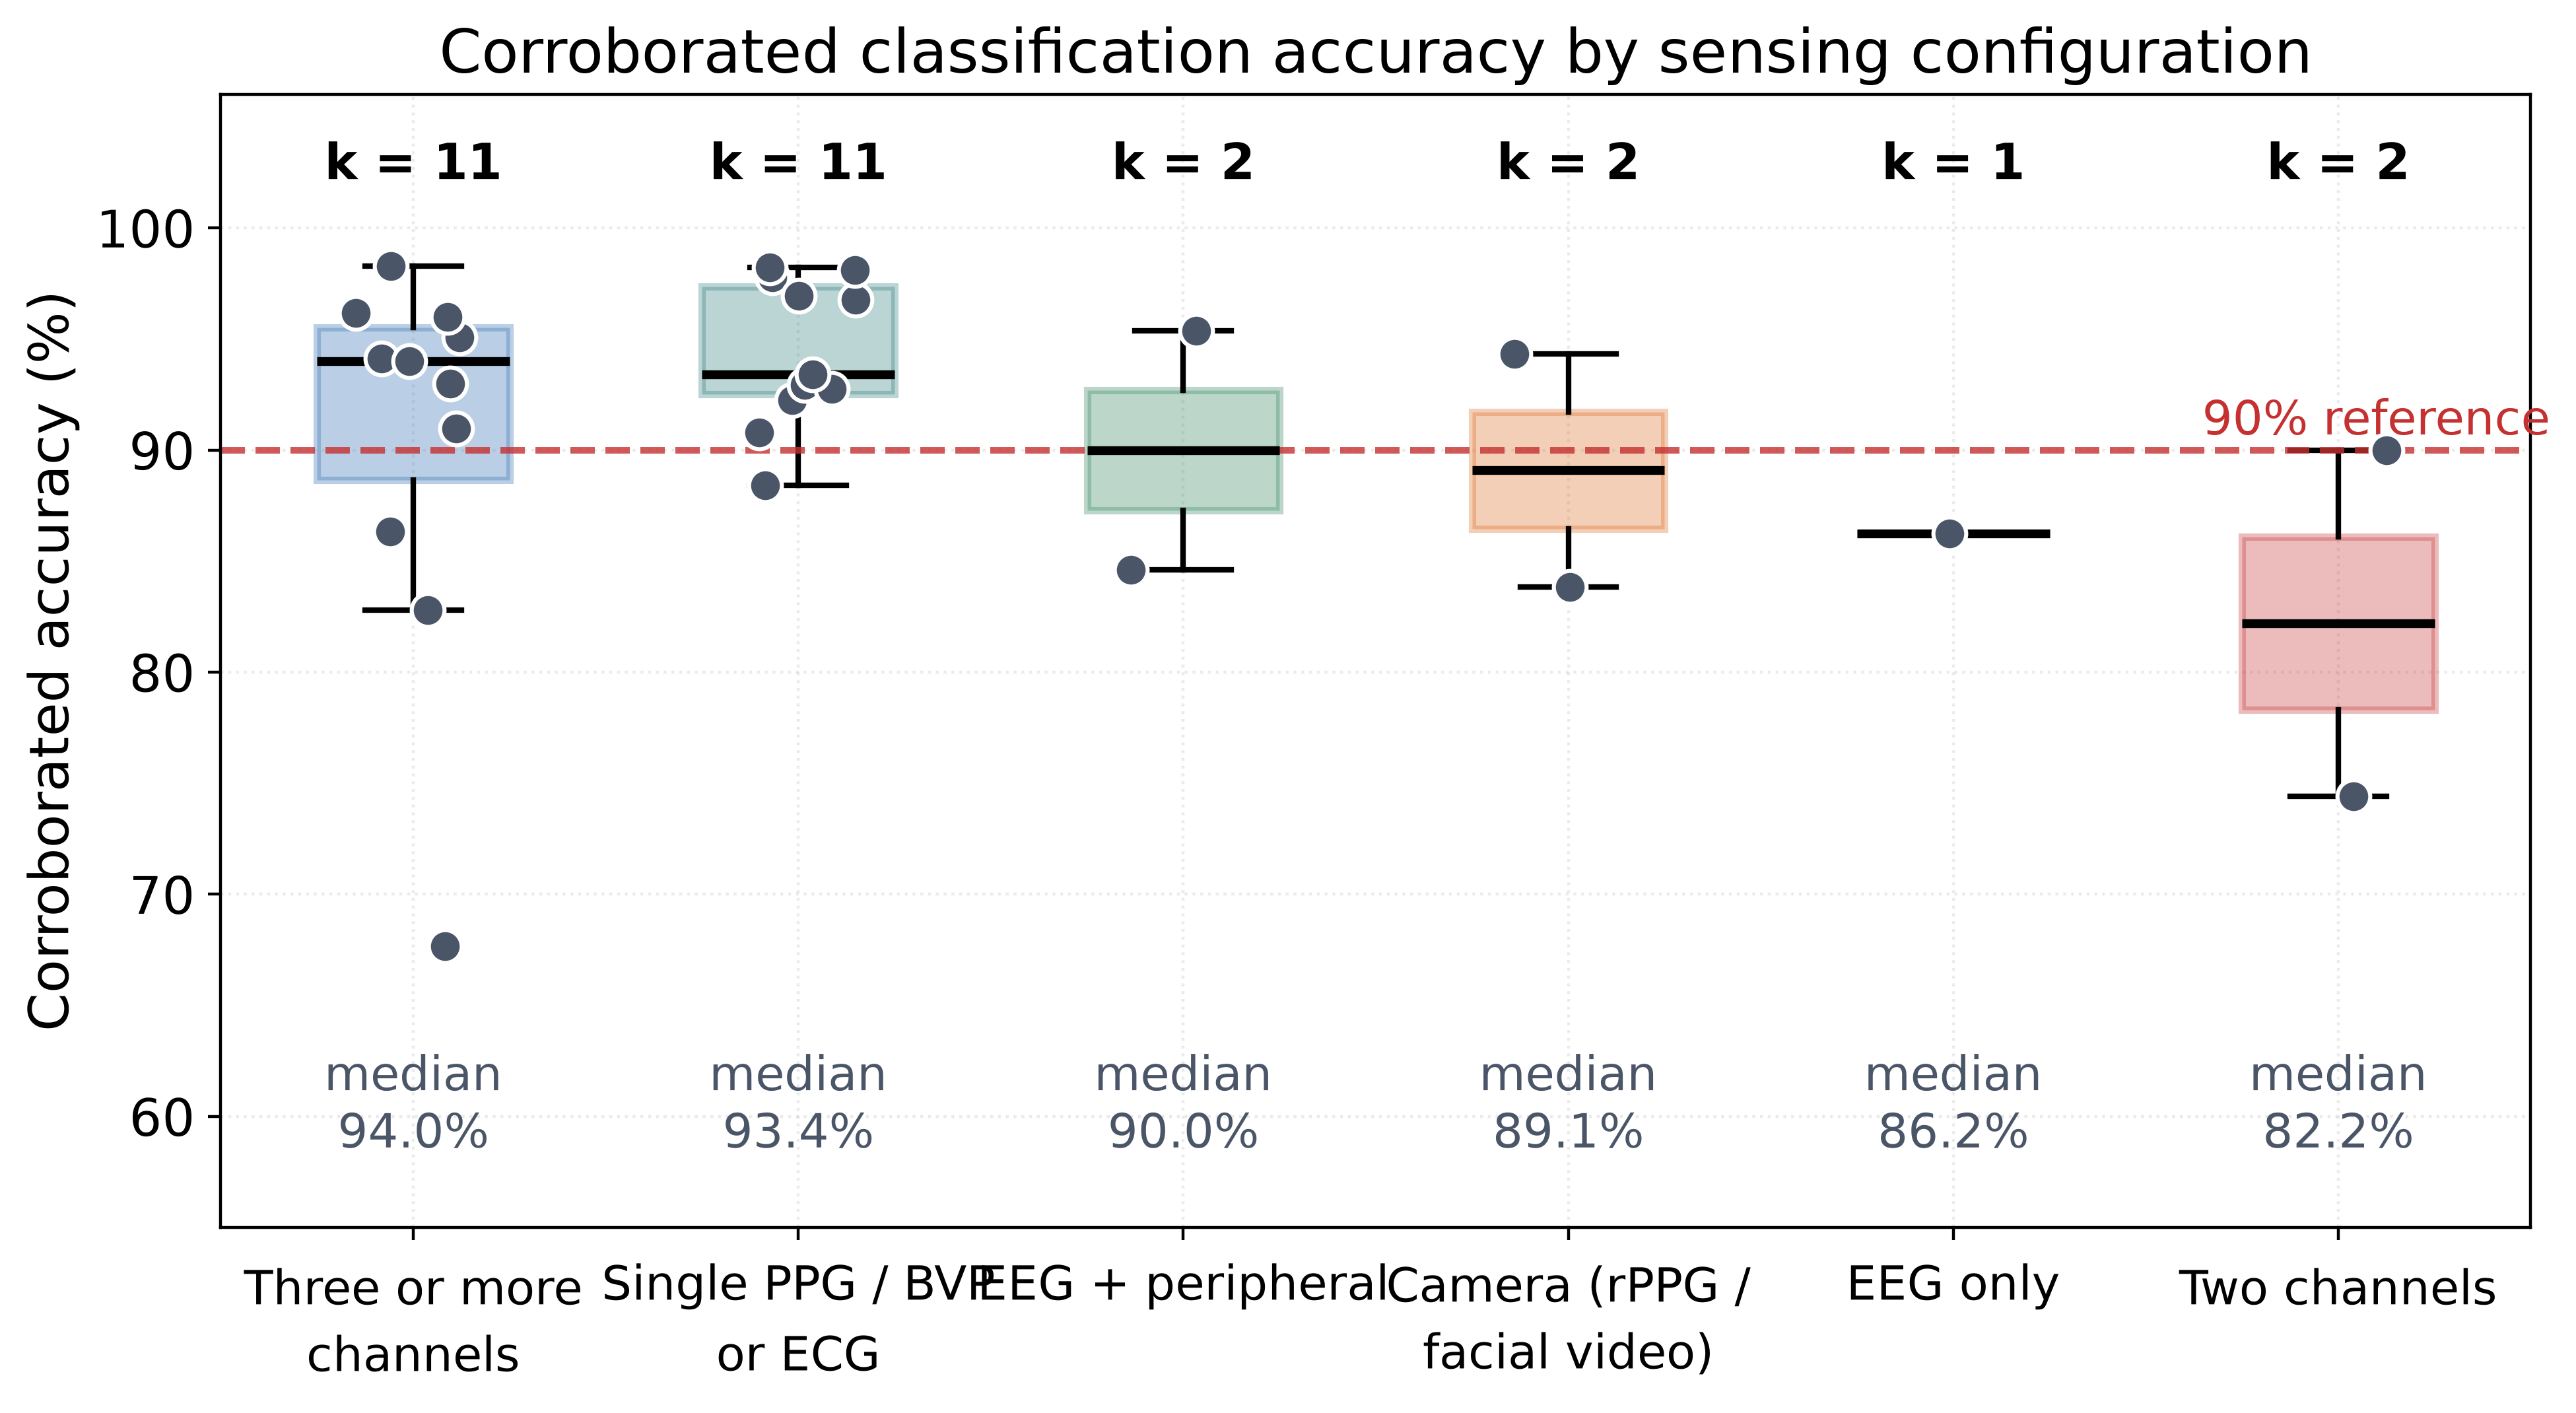
\includegraphics[width=0.86\textwidth]{fig5_modality.png}
\caption{Corroborated classification accuracy grouped by sensing configuration. Boxes show
the median and interquartile range, individual records are overlaid, and the number of
records $k$ and the group median are annotated. The distributions overlap across
configurations, including between single-channel and three-or-more-channel systems.}
\label{fig:modality}
\end{figure}

\subsubsection{Studies Retained in the Narrative Synthesis}
Thirty-two included studies contribute no numbers because their headline outcome could not be
recovered from the openly retrievable record, yet they define the methodological landscape
that the quantitative findings must be read against. Four themes recur.

\textbf{Architectural elaboration:} Hybrid and generative designs dominate recent output.
A hybrid CNN-transformer with copula-GAN augmentation and Monte Carlo dropout for uncertainty
quantification was evaluated on heart rate and respiratory rate from 34 participants
\cite{r91}; a hybrid CNN-MLP was applied to multi-channel physiological input \cite{r87};
a transformer was applied to five physiological channels from 14 pilots \cite{r42}; a
conditional GAN was used to synthesize physiological time series to address label scarcity
\cite{r70}; and a time-series foundation model was fine-tuned for continuous, explainable
stress monitoring from a wristband \cite{r105}. A study explicitly framed around the
complexity-intrusiveness trade-off compared classical and deep models against how much
daily-life intrusion each device requires \cite{r34}, which is the design question this
review's findings bear on most directly.

\textbf{Deployment constraints:} Several studies target the constraints that matter for
translation rather than accuracy alone. Cost-aware feature selection traded prediction power
against energy, reducing energy cost by up to $94.37\%$ while retaining $90.98\%$ accuracy
\cite{r54}; context-aware selective fusion achieved $2.2\times$ and $2.7\times$ energy
efficiency over conventional fusion on the same hardware \cite{r58}; federated learning was
used to keep wrist EDA on-device \cite{r72}; and secure cloud-connected frameworks were
developed for clinical populations \cite{r51}. Explainability appears both as SHAP and LIME
attribution over deep models \cite{r22} and as genetic-algorithm feature reduction with
Bayesian hyperparameter optimization \cite{r53}.

\textbf{Measurement validity:} A smaller group interrogates whether the signals mean what they
are assumed to mean. Multi-wavelength PPG was validated against microneurography as a
surrogate for stress-induced sympathetic activation \cite{r86}; the relative contribution of
ECG, respiration, GSR and PPG to the stress response was assessed feature by feature, with at
least two statistically significant features recovered from each channel \cite{r29}; salivary
cortisol was used as the reference standard for a context-aware digital biomarker in older
adults \cite{r73}; and rule-based individualised processing of EDA and skin temperature was
proposed in place of a learned model \cite{r48}. Others characterize instrumentation, from
flexible single-lead cardiac electrodes \cite{r76} to multi-parameter assessment platforms
\cite{r41} and wearable bands combining PPG-derived heart rate with GSR \cite{r24}.

\textbf{Generalization as an explicit target:} Three studies treat transfer as the object of
study rather than a limitation. An ensemble of gradient boosting and a neural network trained
on a synthesized 200-subject corpus pooled from SWELL, NEURO, WESAD and UBFC-Phys reported
$25\%$ better predictive performance than singular models, with data and code released
publicly \cite{r101}. Subject-specific baseline normalization against resting state supported
$90.8\%$ accuracy under LOSO validation \cite{r21}. Sleep data from a consumer ring was used
to predict perceived stress longitudinally in first-year students, an outcome regime in which
the achievable performance is far below laboratory figures \cite{r102}. These are the studies
whose design most closely anticipates the conclusions drawn in Sections~4.3 and~4.4.

\subsection{Benchmark Saturation}
WESAD is the reference dataset of this literature and supplies 10 of the 34 corroborated
outcome records. Figure~\ref{fig:wesad} examines what those records actually discriminate.
Figure~\ref{fig:wesad}(a) ranks every corroborated WESAD result by accuracy and colors each
by validation protocol; Figure~\ref{fig:wesad}(b) stratifies the same records by protocol.

Excluding the single subject-independent generalized evaluation, 9 records span
$86.34\%$ to $98.23\%$ and 7 of those 9 exceed $92\%$. That band is occupied indiscriminately
by a context-aware wrist ensemble \cite{r58}, a capsule network on HRV features \cite{r61}, a
$k$-nearest-neighbour classifier on 65 handcrafted features \cite{r14}, a residual
transformer on blood volume pulse \cite{r50} and a transpose-enhanced autoencoder \cite{r55}.
A classical KNN pipeline at $96.00\%$ \cite{r14} is not meaningfully separated from a
transformer at $98.23\%$ \cite{r50}. When architectures spanning two decades of methodological
development are compressed into two percentage points, the benchmark is no longer measuring
architecture.

Figure~\ref{fig:wesad}(b) makes the more consequential point. The median of the records whose
protocol was never stated is $95.06\%$, and the median of the records explicitly validated
leave-one-subject-out is $94.59\%$. These are indistinguishable, which means protocol
reporting on WESAD currently carries almost no information. The single record evaluated as a
subject-independent generalized model falls to $67.65\%$ \cite{r33}, more than 27 pp below
every other record on the same dataset. The saturation is therefore not uniform: WESAD is
saturated for subject-dependent and LOSO evaluation and remains far from saturated for
genuine subject-independent generalization, which is the regime relevant to deployment and
the one almost nobody reports.

\begin{figure}[H]
\centering
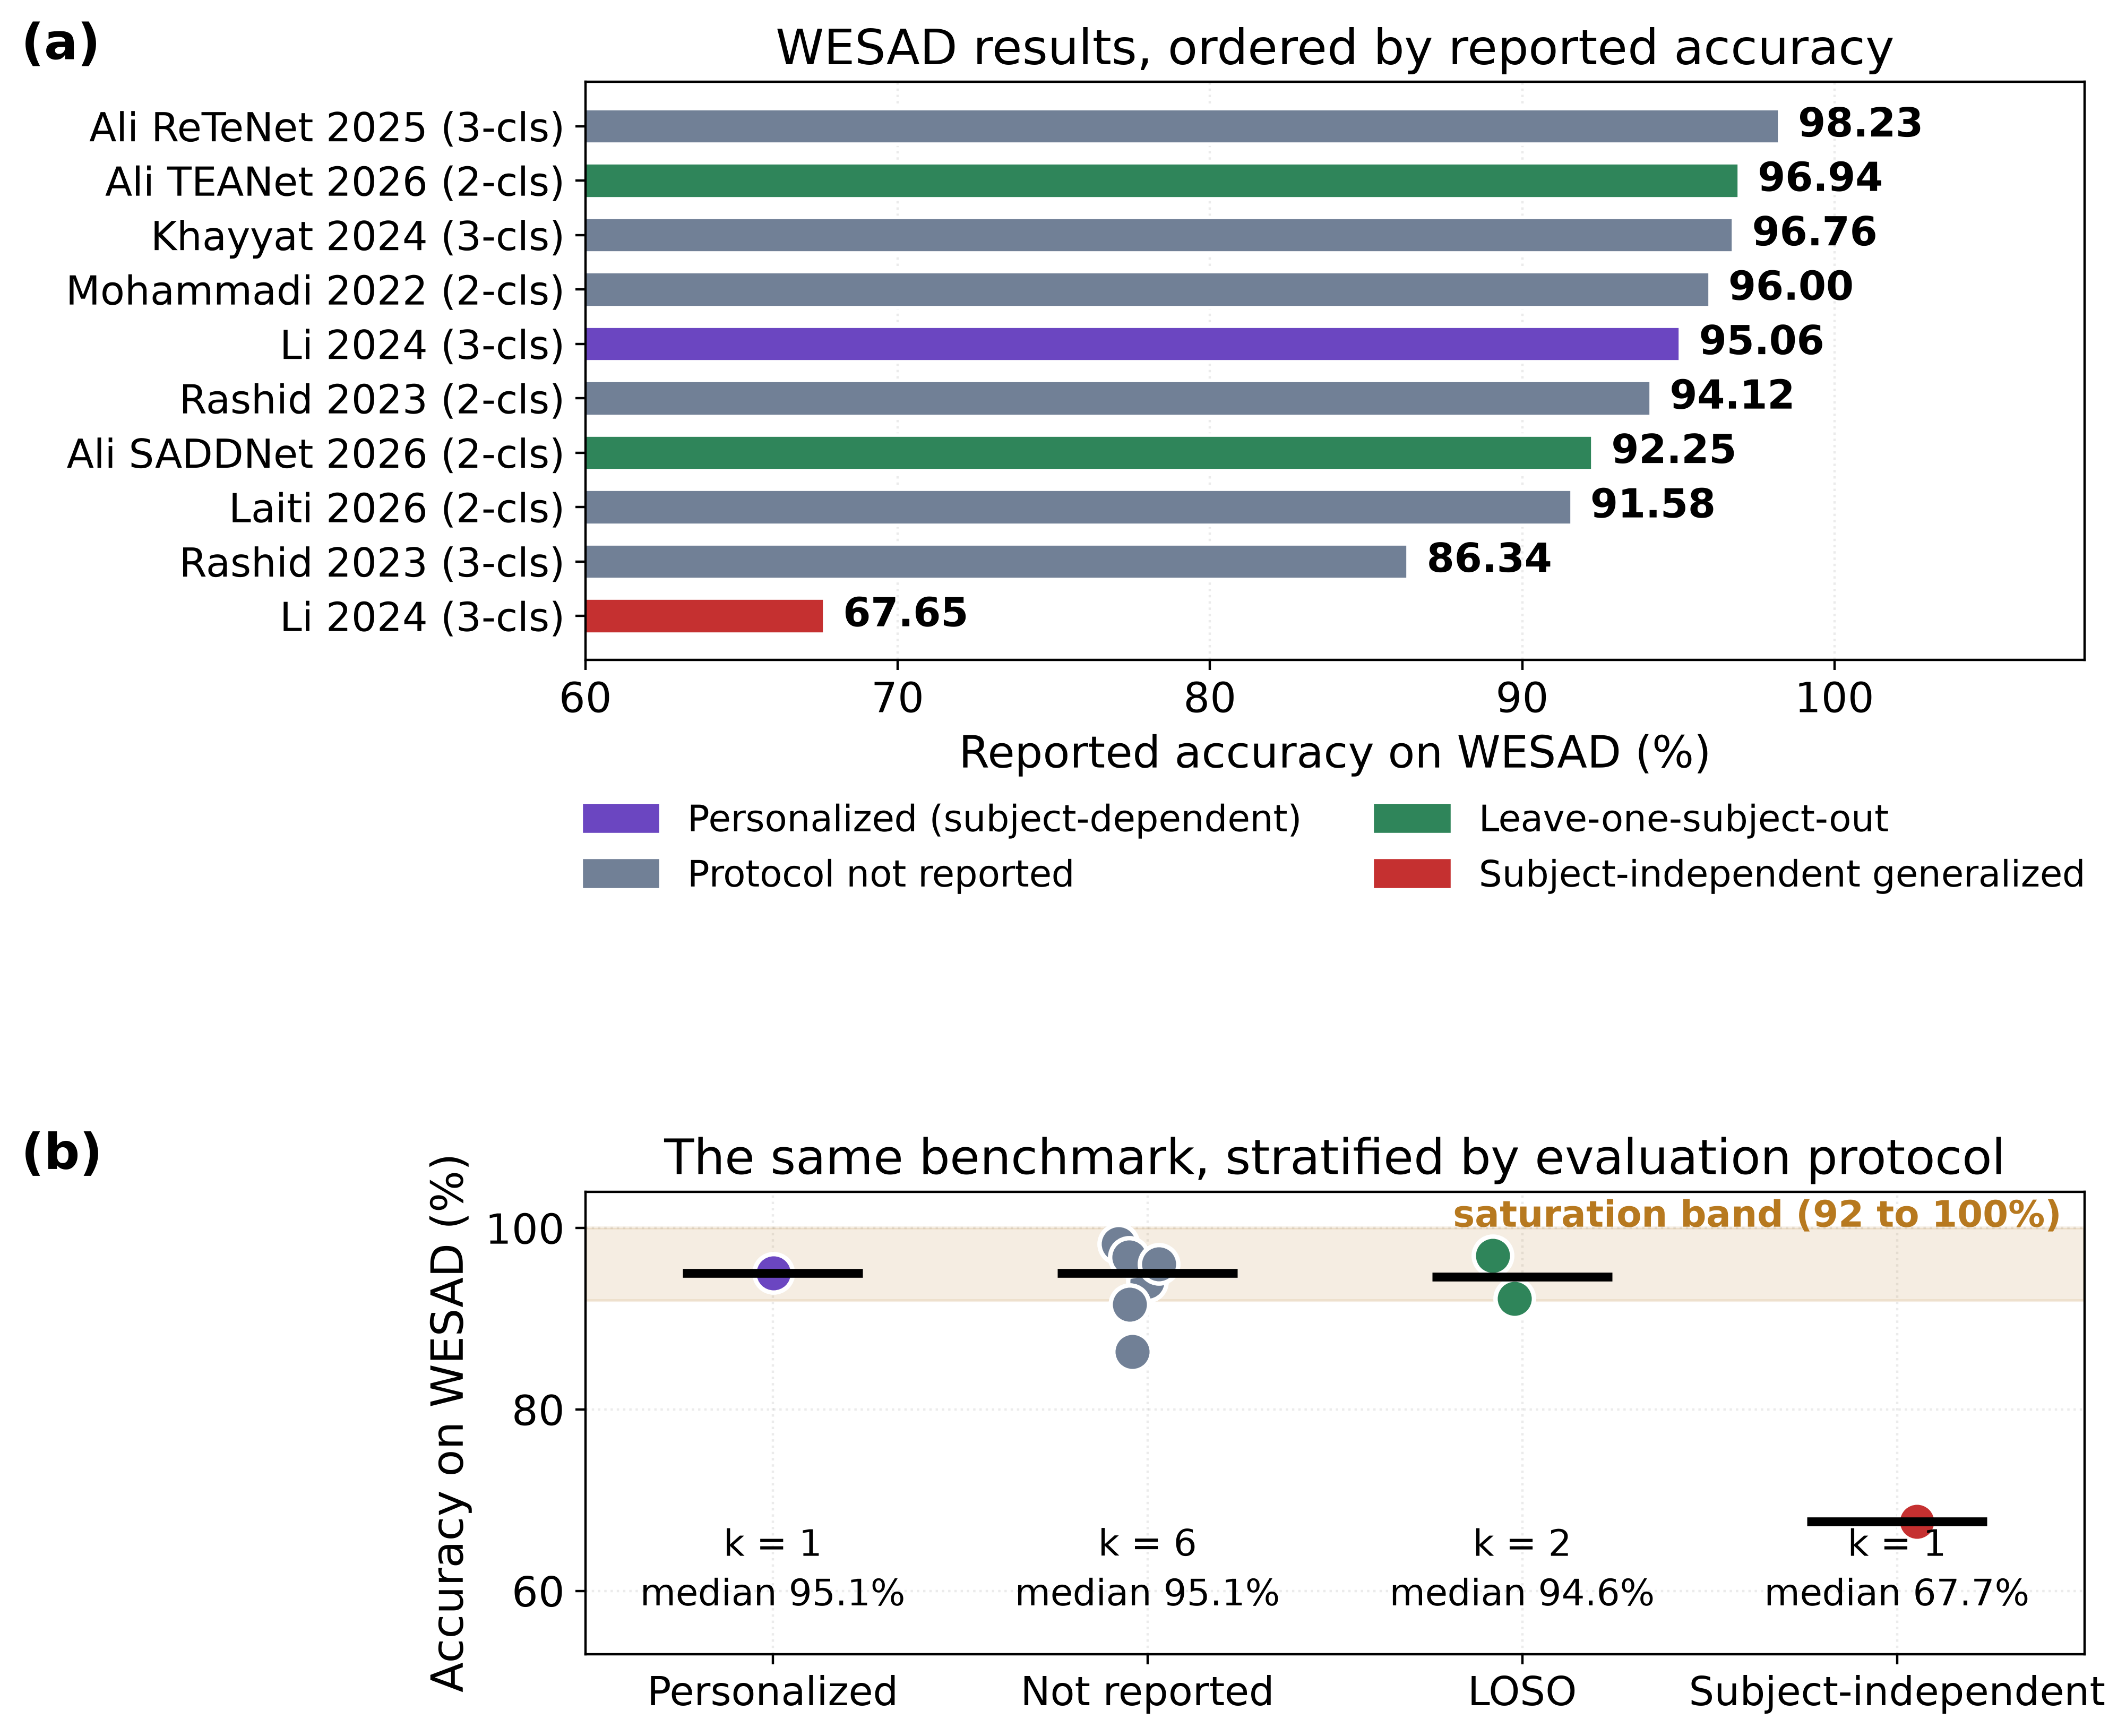
\includegraphics[width=0.99\textwidth]{fig6_wesad.png}
\caption{Saturation of the WESAD benchmark. Figure~\ref{fig:wesad}(a) ranks all corroborated
WESAD records by reported accuracy, with each bar colored by the validation protocol and the
number of classes given in the label. Figure~\ref{fig:wesad}(b) stratifies the same records by
protocol, showing individual records, the group median as a horizontal rule, and the
saturation band between 92 and 100\%. Personalized and protocol-unreported records are
indistinguishable from leave-one-subject-out records, while the single subject-independent
generalized evaluation falls far below all of them.}
\label{fig:wesad}
\end{figure}

\subsection{Within-Study Fusion Gain}
Four studies in the corpus report a single-modality baseline and a multimodal result on the
same cohort, with the same pipeline and under the same validation protocol.
Table~\ref{tab:t5} gives these contrasts and Figure~\ref{fig:fusion} displays them.

\begin{table}[H]
\centering
\caption{Within-study, protocol-matched contrasts between the best single modality and the
multimodal configuration. Each row holds cohort, pipeline and validation protocol fixed, so
the difference is attributable to the added modality. Gains in the AUROC row are expressed in
percentage points of AUROC and are not pooled with the accuracy rows.}
\label{tab:t5}
\small
\resizebox{\textwidth}{!}{\begin{tabular}{L{3.2cm} L{2.25cm} L{2.8cm} L{1.9cm} C{0.7cm} C{1.4cm} C{1.4cm} C{1.3cm}}
\toprule
\textbf{Study} & \textbf{Single modality} & \textbf{Multimodal configuration} & \textbf{Fusion level} & \textbf{$n$} & \textbf{Unimodal} & \textbf{Multimodal} & \textbf{Gain (pp)} \\
\midrule
Abdul Kader et al. \cite{r75} & EEG & EEG+GSR & Feature-level & 20 & 70.30 & 84.60 & $+$14.30 \\
Campanella et al. \cite{r12} & PPG (HR) & PPG+EDA & Feature-level & 29 & 83.89 & 90.00 & $+$6.11 \\
Awada et al. \cite{r26} & Physiological & Physiological + behavioral & Decision-level & NR & 79.55 & 82.78 & $+$3.23 \\
Kim et al. \cite{r37} & GSR & EEG+GSR & Feature-level & 30 & 94.40 & 95.40 & $+$1.00 \\
\midrule
\multicolumn{7}{l}{\textbf{Median gain} (range 1.00 to 14.30, $k=4$)} & \textbf{$+$4.67} \\
\bottomrule
\end{tabular}}
\end{table}

\begin{figure}[H]
\centering
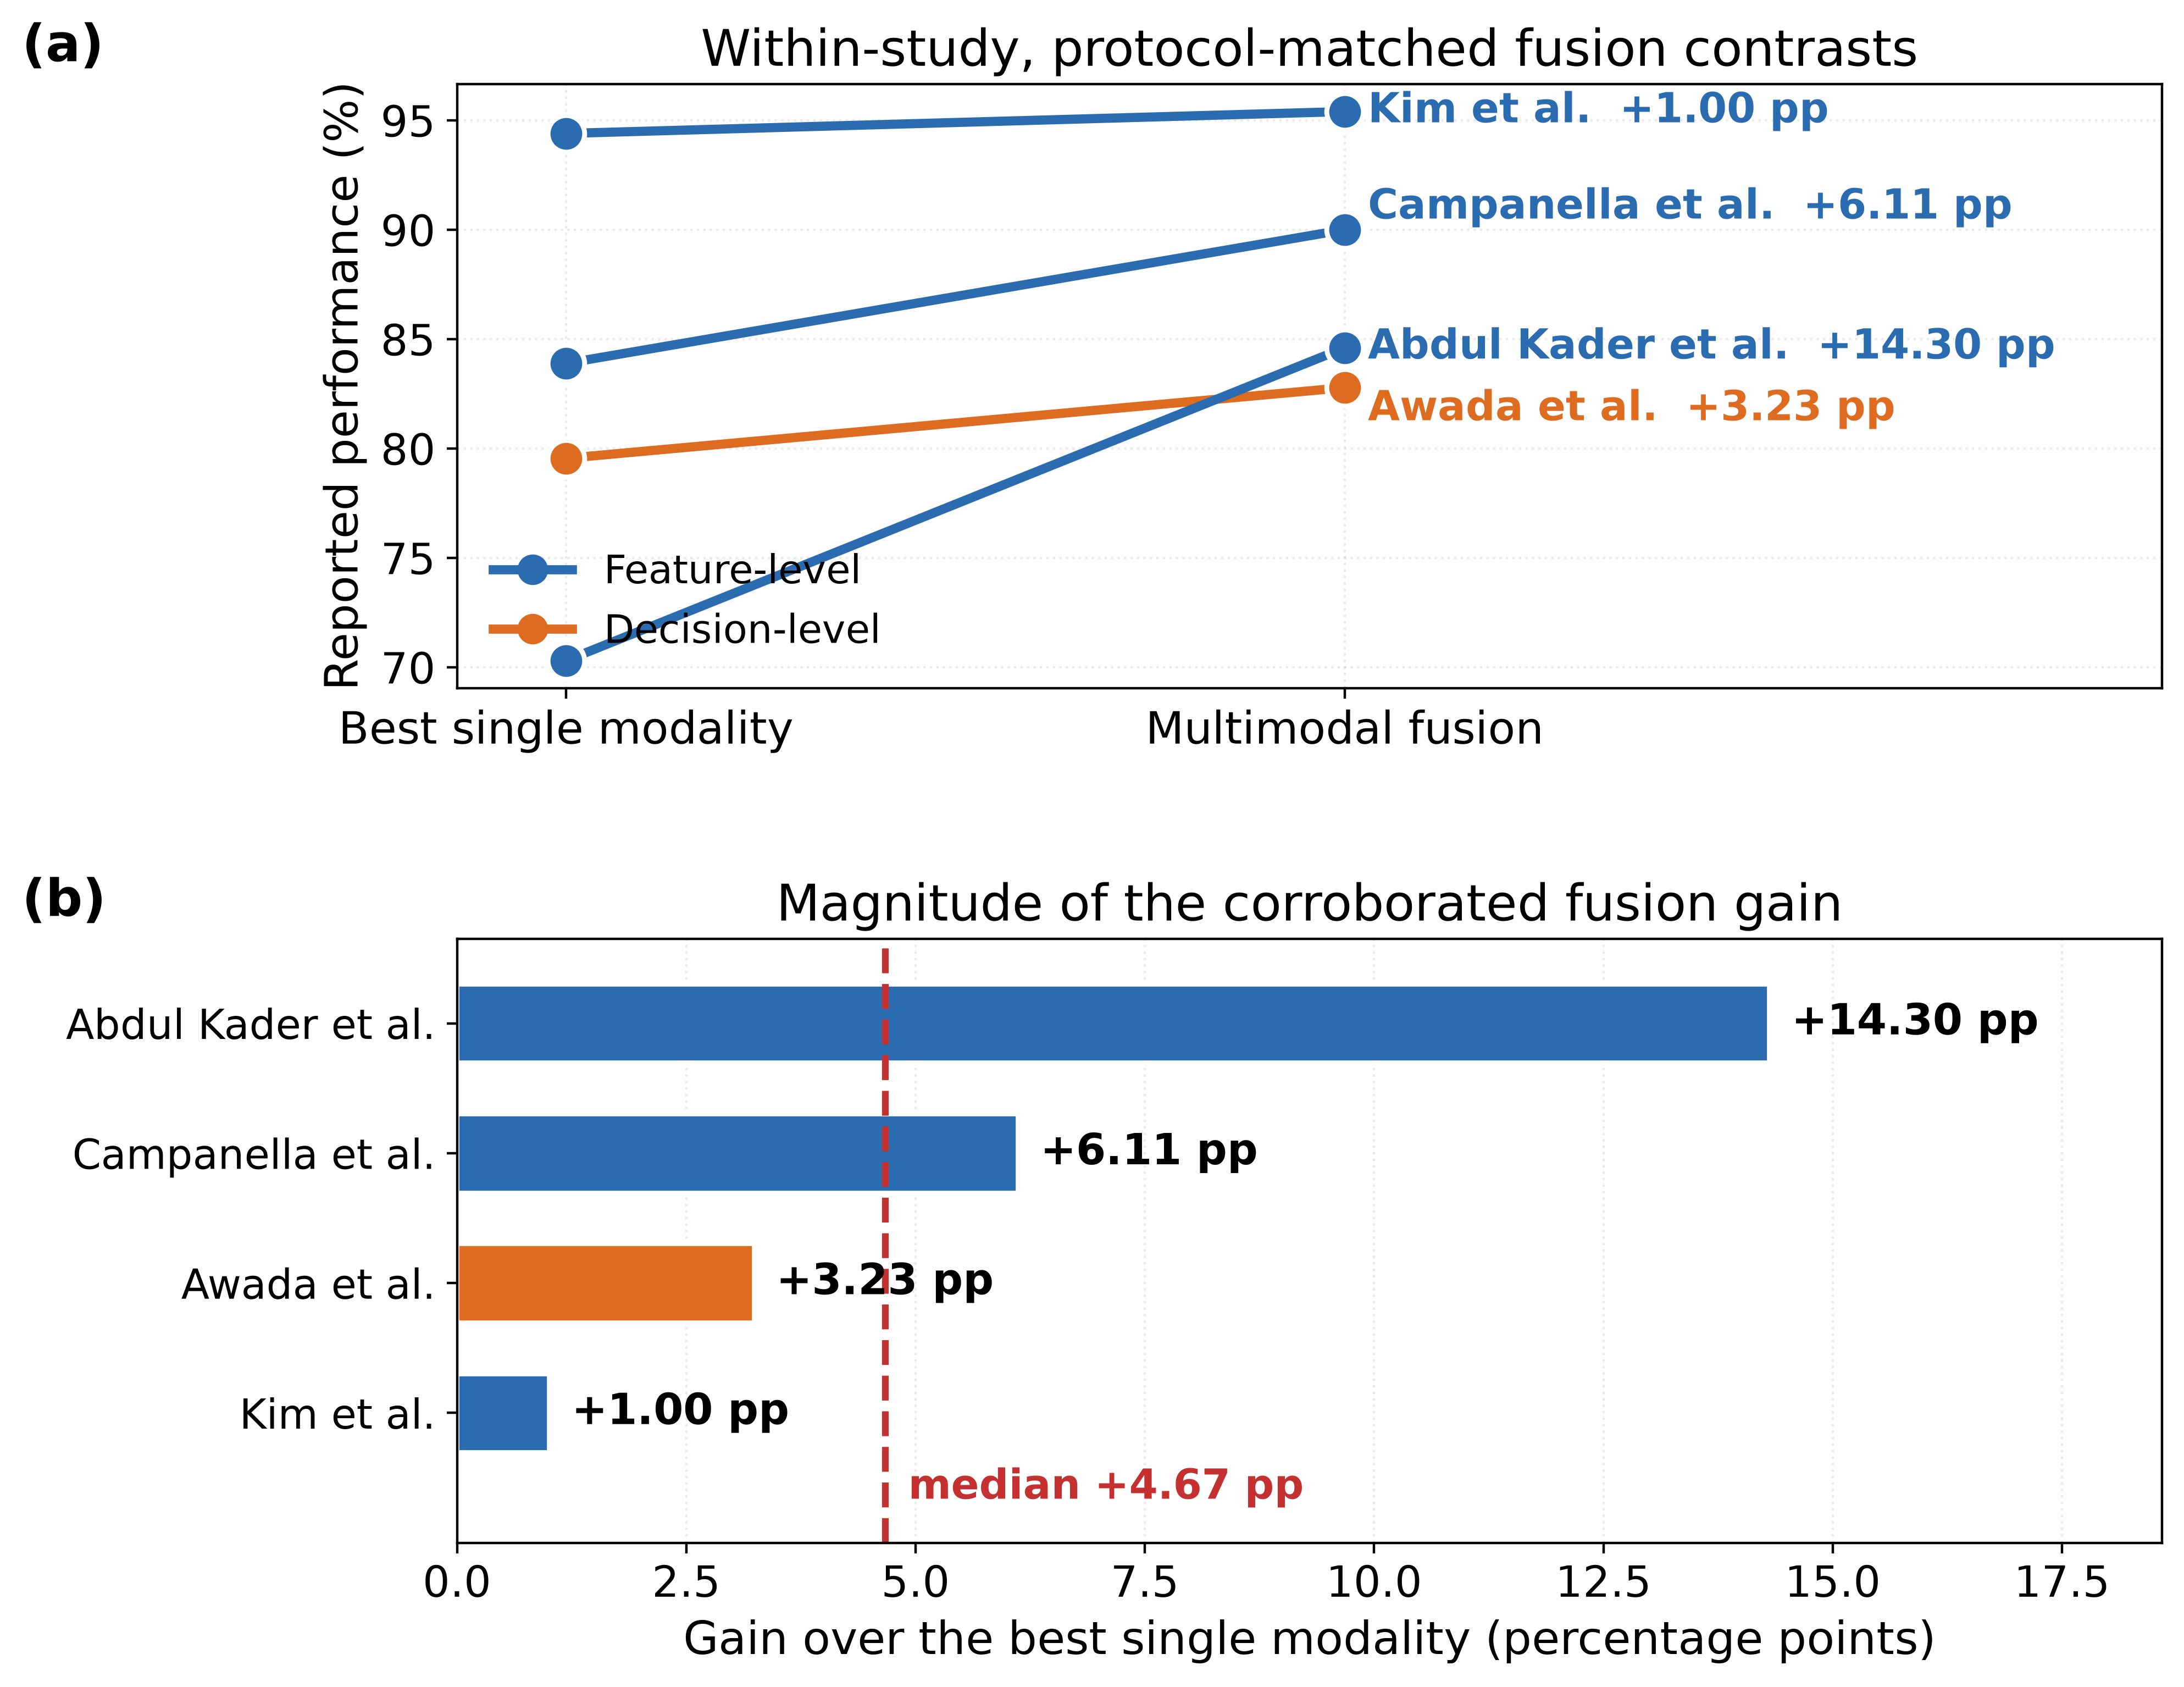
\includegraphics[width=0.99\textwidth]{fig7_fusion.png}
\caption{Within-study fusion gain. Figure~\ref{fig:fusion}(a) shows each study as a line
connecting its best single-modality result to its multimodal result under an identical
protocol, colored by fusion level. Figure~\ref{fig:fusion}(b) shows the magnitude of each
gain against the median across the four contrasts.}
\label{fig:fusion}
\end{figure}

Every contrast is positive, so fusion does help. The magnitude, however, is modest and highly
uneven. The median gain is $+4.67$ pp, and the range spans $+1.00$ to $+14.30$ pp. The
largest gain, $+14.30$ pp, comes from adding galvanic skin response to a single EEG channel
\cite{r75}, where the baseline modality is weak at $70.30\%$ and the added channel is
physiologically distinct. The smallest, $+1.00$ pp of AUROC, comes from adding EEG to GSR
\cite{r37}, where the baseline is already strong at $0.944$ and fusion adds little headroom.
Adding facial and behavioral features to a physiological wristband in an office cohort
yields $+3.23$ pp, from $79.55\%$ to $82.78\%$ \cite{r26}; notably, the authors of that study
themselves conclude that the small difference indicates physiological data alone may be
adequate for their task. Adding EDA to heart rate gives $+6.11$ pp \cite{r12}.

A coherent pattern emerges. Fusion gain is largest where the unimodal baseline is weakest and
where the added channel is physiologically non-redundant, and it approaches zero as the
baseline strengthens. This is the behavior expected of a complementary-information effect
operating against a ceiling, and it means that headline fusion gains harvested from
weak-baseline studies do not transfer to systems whose unimodal baseline is already strong.

\subsection{Within-Study Evaluation-Induced Gaps}
Ten within-study contrasts isolate the effect of an evaluation choice while holding the model
and data-generating process fixed. Table~\ref{tab:t6} lists them and
Figure~\ref{fig:protocol} compares them against the fusion gains of Section~4.3 on a common
scale.

\begin{table}[H]
\centering
\caption{Within-study contrasts attributable to evaluation choices. Each row reports the same
model or pipeline under a more favorable and a more realistic evaluation condition. The
final rows give the median gap alongside the median within-study fusion gain for direct
comparison.}
\label{tab:t6}
\small
\resizebox{\textwidth}{!}{\begin{tabular}{L{3.1cm} L{4.35cm} L{2.35cm} C{1.2cm} C{1.4cm} C{1.4cm} C{1.3cm}}
\toprule
\textbf{Study} & \textbf{Contrast} & \textbf{Source of the difference} & \textbf{Metric} & \textbf{Favourable} & \textbf{Realistic} & \textbf{Gap (pp)} \\
\midrule
Li \& Washington \cite{r33} & Personalized vs subject-independent & Personalization & F1 & 91.71 & 43.05 & 48.66 \\
Li \& Washington \cite{r33} & Personalized vs subject-independent & Personalization & Accuracy & 95.06 & 67.65 & 27.41 \\
Laiti et al. \cite{r49} & WESAD vs Wellby real-world cohort & Dataset transfer & AUROC & 91.58 & 77.02 & 14.56 \\
Toshnazarov et al. \cite{r13} & Laboratory vs free-living & Deployment setting & F1 & 84.00 & 71.00 & 13.00 \\
Xu et al. \cite{r16} & Stress state vs stress level & Task granularity & Accuracy & 94.33 & 83.83 & 10.50 \\
Rashid et al. \cite{r58} & Binary vs three-class & Task granularity & Accuracy & 94.12 & 86.34 & 7.78 \\
Ali et al. \cite{r55} & WESAD vs in-house cohort & Dataset transfer & Accuracy & 96.94 & 92.94 & 4.00 \\
Khayyat et al. \cite{r61} & WESAD vs SWELL-KW & Dataset transfer & Accuracy & 96.76 & 92.76 & 4.00 \\
Khayyat et al. \cite{r61} & Binary vs multiclass (WESAD) & Task granularity & Accuracy & 99.82 & 96.76 & 3.06 \\
Shikha et al. \cite{r53} & Two-level vs three-level stress & Task granularity & Accuracy & 98.28 & 97.02 & 1.26 \\
\midrule
\multicolumn{6}{l}{\textbf{Median evaluation-induced gap} (range 1.26 to 48.66, $k=10$)} & \textbf{9.14} \\
\multicolumn{6}{l}{Median within-study fusion gain for comparison ($k=4$)} & 4.67 \\
\bottomrule
\end{tabular}}
\end{table}

\begin{figure}[H]
\centering
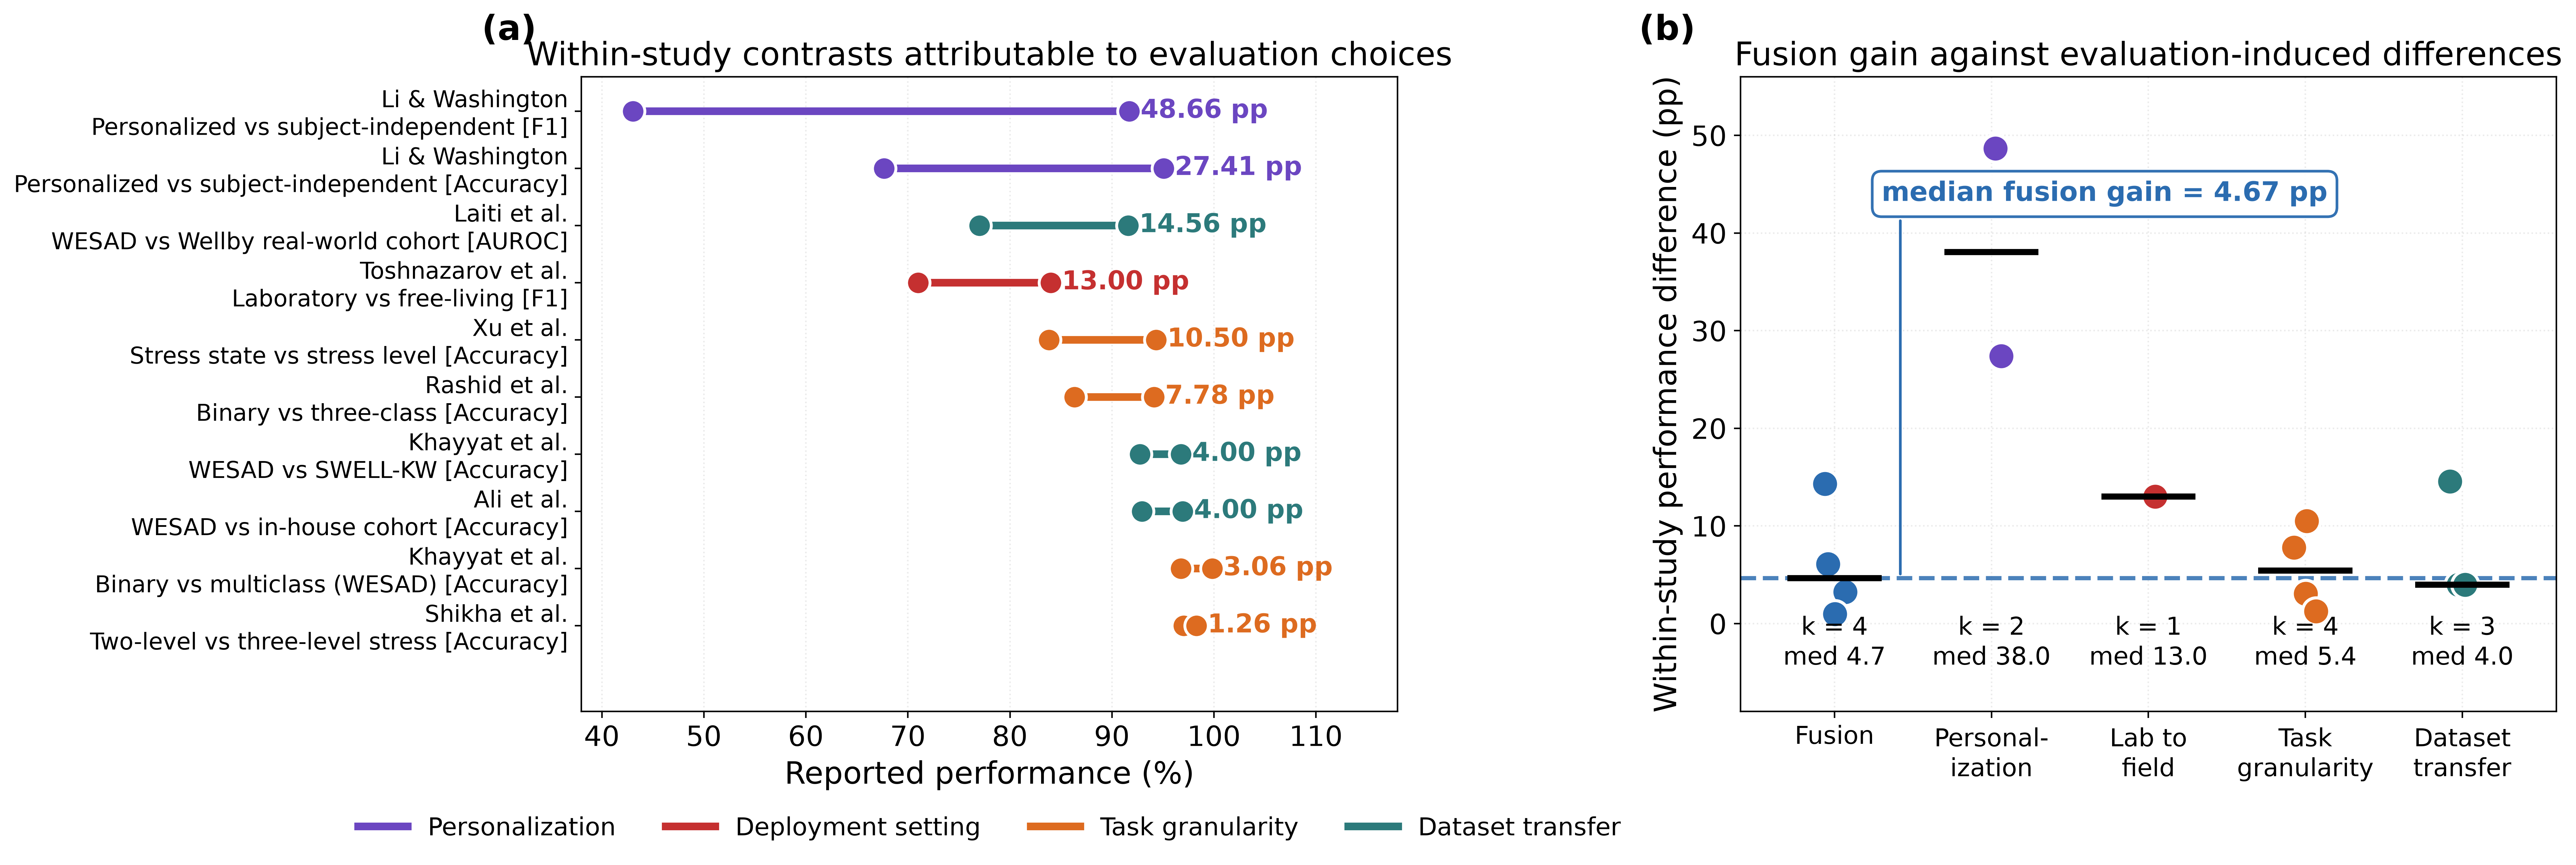
\includegraphics[width=0.99\textwidth]{fig8_protocol_vs_fusion.png}
\caption{Evaluation effects against fusion effects. Figure~\ref{fig:protocol}(a) shows each
within-study evaluation contrast as a segment joining the favorable and the realistic
condition, colored by the source of the difference and annotated with the gap in percentage
points. Figure~\ref{fig:protocol}(b) places the four within-study fusion gains and the four
families of evaluation contrast on a common axis, with group medians shown as horizontal
rules and the median fusion gain marked by the dashed line.}
\label{fig:protocol}
\end{figure}

The median evaluation-induced gap is $9.14$ pp, approximately twice the median fusion gain of
$4.67$ pp, and the four families differ sharply in severity.

\textbf{Personalization:} This is the dominant effect in the corpus, with a median gap of
$38.03$ pp. In a single study using consumer wearable data for three-class affect
classification, a personalized model reached $95.06\%$ accuracy with an F1 of $91.71$, while
the subject-exclusive generalized model on the same data reached $67.65\%$ with an F1 of
$43.05$ \cite{r33}. The accuracy gap of $27.41$ pp is $5.9$ times the median fusion gain, and
the F1 gap of $48.66$ pp is $10.4$ times it. The F1 collapse is the more diagnostic figure:
it indicates that the generalized model is not merely less accurate but is failing on the
minority classes that matter, which an accuracy figure partially conceals.

\textbf{Deployment setting:} Moving from controlled laboratory recording to free living cost
$13.00$ pp of F1 in a smartwatch study that evaluated both, falling from $0.84$ to $0.71$
\cite{r13}. That single study is worth more for deployment planning than any number of
laboratory accuracy figures, and it is nearly three times the median fusion gain.

\textbf{Dataset transfer:} Three contrasts give a median of $4.00$ pp, but the range is
instructive. Transfer between two curated laboratory benchmarks is cheap: $4.00$ pp between
WESAD and SWELL-KW \cite{r61} and $4.00$ pp between WESAD and an in-house cohort under
matched LOSO validation \cite{r55}. Transfer from a benchmark to a genuine real-world student
cohort is not: AUROC fell from $91.58$ on WESAD to $77.02$ in a real-world deployment, a gap
of $14.56$ pp \cite{r49}. Benchmark-to-benchmark transfer therefore substantially
underestimates benchmark-to-field transfer, and reporting the former as evidence of
generalization is misleading.

\textbf{Task granularity:} Four contrasts give a median of $5.42$ pp. Binary stress detection
exceeds three-class detection by $7.78$ pp in one wrist-based ensemble \cite{r58}, binary
stress state exceeds graded stress level by $10.50$ pp in a facial video system \cite{r16},
and smaller penalties of $3.06$ pp \cite{r61} and $1.26$ pp \cite{r53} appear elsewhere. Since
clinical and operational utility generally requires graded rather than binary output, the
binary figures that dominate the literature systematically overstate deployable performance.

\subsection{Cohort Size, Transfer and Reporting}
Figure~\ref{fig:transfer} examines two further properties of the evidence base.
Figure~\ref{fig:transfer}(a) shows the three contrasts in which a model was evaluated both on
its development condition and on a transfer condition. Figure~\ref{fig:transfer}(b) plots
corroborated accuracy against evaluation cohort size on a logarithmic axis.

\begin{figure}[H]
\centering
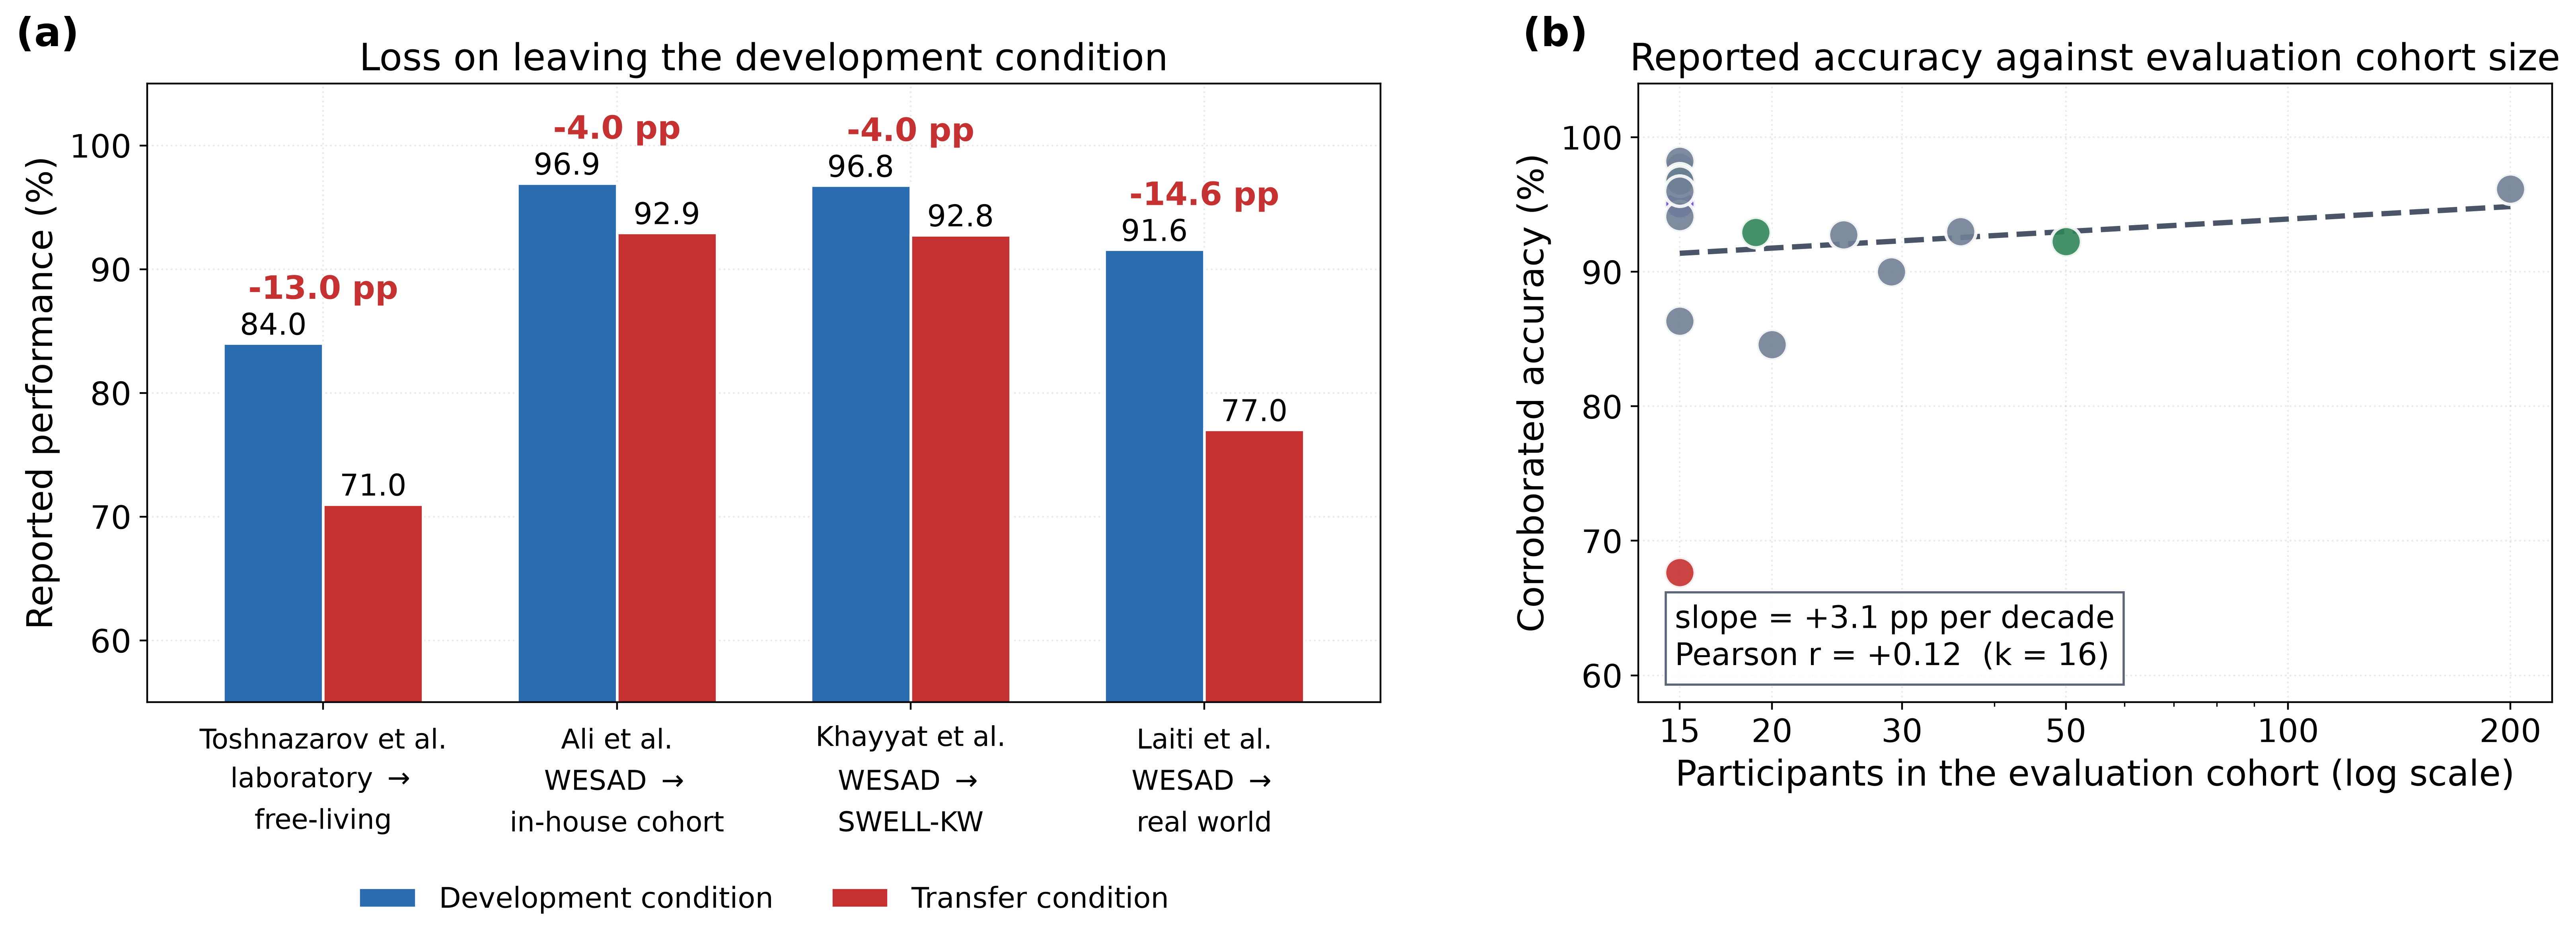
\includegraphics[width=0.99\textwidth]{fig9_transfer.png}
\caption{Transfer behavior and the absence of a cohort-size effect.
Figure~\ref{fig:transfer}(a) contrasts performance on the development condition with
performance on the transfer condition for the three studies reporting both, annotated with
the loss in percentage points. Figure~\ref{fig:transfer}(b) plots corroborated accuracy
against the number of participants in the evaluation cohort on a logarithmic axis, with
points colored by validation protocol and a least-squares fit on the log axis.}
\label{fig:transfer}
\end{figure}

The relationship between cohort size and reported accuracy is essentially flat
($r=+0.15$, slope $+3.7$ pp per decade, $k=15$). Studies evaluating on 15 participants report
accuracies indistinguishable from studies evaluating on 200. Under any reasonable model of
task difficulty, a larger and more heterogeneous cohort should be harder, so a flat or
slightly positive relationship is not evidence that small studies are adequate; it is
evidence that reported accuracy is being set by evaluation design rather than by the
difficulty of the underlying problem.

Figure~\ref{fig:verify} reports the verification and reporting audit.
Figure~\ref{fig:verify}(a) shows that a headline outcome could be independently corroborated
for 28 of 60 included studies (46.7\%). Figure~\ref{fig:verify}(b) shows recovery rates for
each reporting item: the evaluation cohort size was recoverable for 18 studies (30.0\%),
whether a public benchmark was used for 14 (23.3\%), the validation protocol for 8 (13.3\%)
and any variance or confidence interval for only 3 (5.0\%).

\begin{figure}[H]
\centering
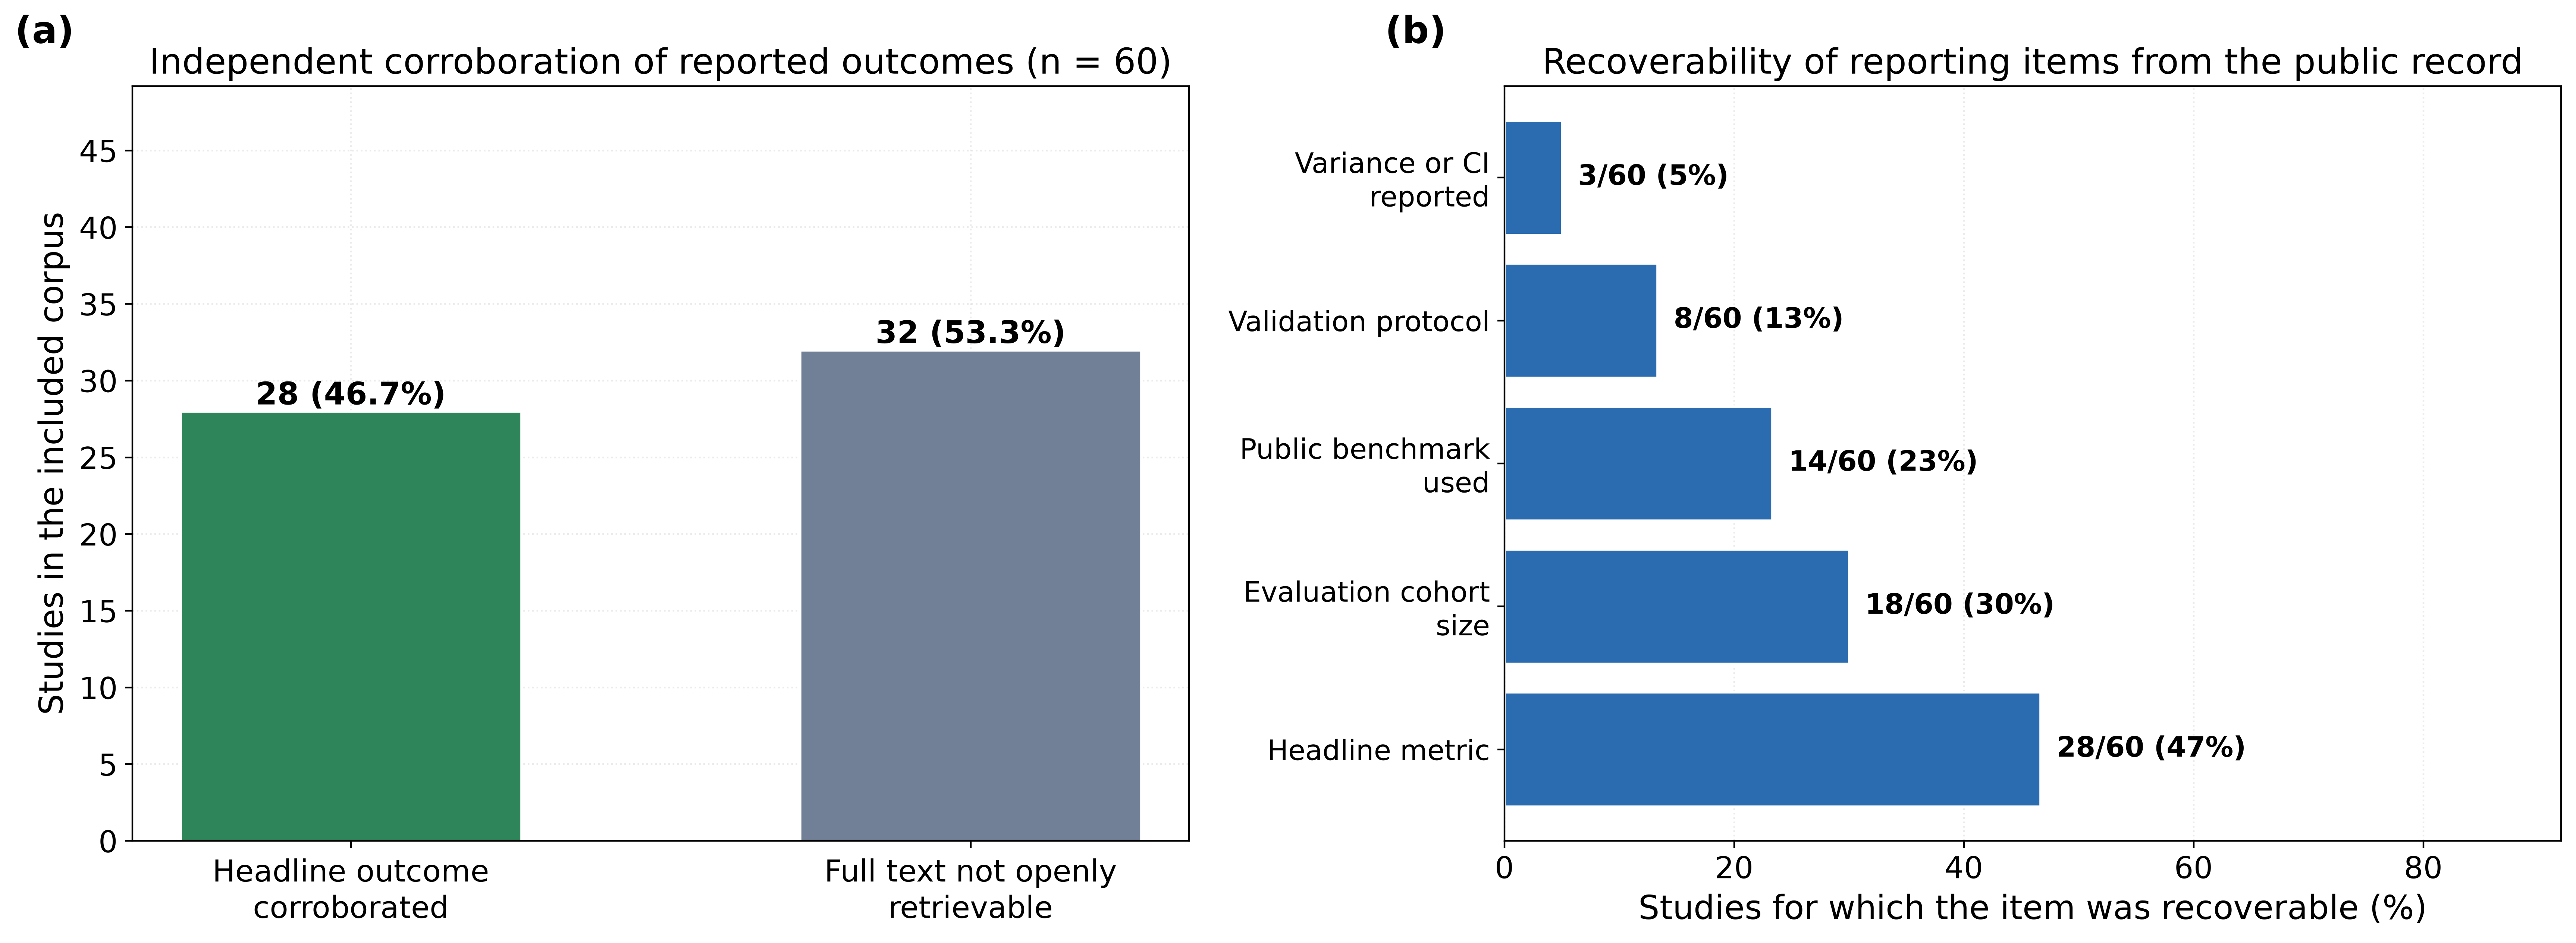
\includegraphics[width=0.99\textwidth]{fig10_verifiability.png}
\caption{Verification and reporting audit across all 60 included studies.
Figure~\ref{fig:verify}(a) shows the proportion of studies for which a headline outcome could
be independently corroborated from the openly retrievable record.
Figure~\ref{fig:verify}(b) shows the recovery rate for each of the five reporting items,
with the count and percentage annotated.}
\label{fig:verify}
\end{figure}

These rates should be read as a property of the openly retrievable record rather than as a
judgement on the studies, since much of the corpus sits behind subscription access. The
implication is nevertheless concrete and is the central practical finding of
Section~4.4: for roughly seven studies in eight, a reader without subscription access cannot
determine the validation protocol, and therefore cannot determine whether a quoted accuracy
describes subject-dependent or subject-independent performance. Given that this single
distinction is worth up to $27.41$ pp of accuracy and $48.66$ pp of F1 within one study
\cite{r33}, an unlabeled accuracy figure in this literature carries very little information.

\begin{table}[H]
\centering
\caption{Constraints on deployment, the corroborated quantitative evidence for each, and its
implication. Only effects supported by a within-study contrast or a directly corroborated
value are listed; magnitudes are those reported in Tables~\ref{tab:t5} and~\ref{tab:t6}.}
\label{tab:t7}
\small
\resizebox{\textwidth}{!}{%
\begin{tabular}{L{2.9cm} L{5.15cm} C{2.3cm} L{5.35cm}}
\toprule
\textbf{Constraint} & \textbf{Corroborated evidence} & \textbf{Magnitude} &
\textbf{Implication for deployment} \\
\midrule
Subject heterogeneity & Personalized versus subject-exclusive generalized model on identical
  data \cite{r33} & 27.41 pp accuracy; 48.66 pp F1 & Calibration data per user is the single
  highest-value design decision; generalized models must not be specified from personalized
  results. \\
Ecological validity & Laboratory versus free-living F1 in the same smartwatch study
  \cite{r13} & 13.00 pp F1 & Laboratory accuracy is not an upper bound that degrades
  gracefully; field validation is required before any deployment claim. \\
Benchmark-to-field transfer & WESAD AUROC versus real-world student cohort AUROC
  \cite{r49} & 14.56 pp AUROC & Benchmark-to-benchmark transfer (4.00 pp) understates
  benchmark-to-field transfer by roughly a factor of three. \\
Output granularity & Binary versus graded outputs across four studies
  \cite{r16,r53,r58,r61} & 5.42 pp median & Binary benchmarks overstate the performance of
  the graded outputs that clinical and operational use requires. \\
Benchmark saturation & 7 of 9 non-subject-independent WESAD records above 92\%, spanning KNN
  to transformers \cite{r14,r50,r55,r58,r61} & $<$ 2 pp separating classical from
  transformer models & WESAD can no longer adjudicate between architectures; new
  architectural claims need a harder or subject-independent evaluation. \\
Reporting completeness & Validation protocol recoverable for 8 of 60 studies; variance for 3
  of 60 & 13.3\%; 5.0\% & Most reported accuracies cannot be interpreted, and meta-analytic
  pooling across this literature is not currently defensible. \\
Modality redundancy & Fusion gain shrinks as the unimodal baseline strengthens
  \cite{r12,r26,r37,r75} & $+1.00$ to $+14.30$ pp & Sensor count should be justified against
  the specific unimodal baseline, not against a generic fusion benefit. \\
\bottomrule
\end{tabular}}
\end{table}

\section{Key Trends and Patterns Across Results}

\subsection{The Field Is Optimizing the Smaller of Two Effects}
The central pattern is a mismatch between where effort is spent and where performance is
determined. Architectural work is abundant: the corpus contains transformers, capsule
networks, autoencoders, generative augmentation and federated schemes, and each reports an
improvement over its chosen baseline. Yet on the one dataset where these architectures can be
compared, they occupy a two-point band that a $k$-nearest-neighbour classifier also occupies
\cite{r14,r50}. Meanwhile the factors that move performance by an order of magnitude more,
whether the model is personalized, whether evaluation is subject independent, whether data
were collected in the field, are treated as reporting details and are usually not reported at
all. A median fusion gain of $4.67$ pp against a median evaluation gap of $9.14$ pp, and
against a personalization gap of $38.03$ pp, quantifies that mismatch.

\subsection{Fusion Is Real, Bounded and Baseline-Dependent}
The four protocol-matched contrasts are unanimously positive, so the case for multimodal
sensing is not overturned. It is bounded. Fusion buys most where the unimodal baseline is
weak and the added channel is physiologically distinct, as in EEG supplemented by GSR at
$+14.30$ pp \cite{r75}, and very little where the baseline is already strong, as in GSR
supplemented by EEG at $+1.00$ pp of AUROC \cite{r37}. Adding a camera channel to a
physiological wristband returned $+3.23$ pp in the one corroborated office deployment
\cite{r26}. For system designers the operational reading is that a second sensor must be
justified against the specific unimodal baseline it will actually replace, together with its
cost in power, cost, form factor and failure modes, and not against a generic claim that
fusion improves performance.

\subsection{Personalization Is the Dominant Lever, and the Main Threat to Validity}
Personalization accounts for the largest effect in the corpus, and simultaneously for the
most serious threat to the interpretability of the literature. Because subject-dependent
splits allow the same participant to appear in training and test, they can be reported
without any deliberate misrepresentation while producing figures that a subject-independent
evaluation would not support. The one study in the corpus that reports both conditions on
identical data shows accuracy falling from $95.06\%$ to $67.65\%$ and F1 from $91.71$ to
$43.05$ \cite{r33}. Since only 8 of 60 studies state their protocol recoverably, the scale of
this effect across the wider literature cannot currently be estimated, which is itself the
finding.

\subsection{Laboratory Performance Does Not Forecast Field Performance}
Two independent within-study contrasts show the same direction and a similar magnitude:
$13.00$ pp of F1 lost between laboratory and free-living conditions \cite{r13}, and
$14.56$ pp of AUROC lost between WESAD and a real-world student cohort \cite{r49}. Transfer
between two curated benchmarks, by contrast, cost only $4.00$ pp \cite{r55,r61}. The gap
between these two figures is the crux: a study that demonstrates cross-dataset transfer
between laboratory corpora has not demonstrated the property that deployment requires. The
structure of the corpus makes this consequential, since 31 of 60 studies are laboratory or
benchmark-only and just 9 involve free-living deployment.

\subsection{Benchmark Saturation Has Made Architectural Claims Unfalsifiable}
When a benchmark compresses a decade of architectural development into a two-point band, it
cannot adjudicate between methods, and improvements reported on it are no longer informative
about which method is better. WESAD has reached that state for subject-dependent and LOSO
evaluation. It has not reached it for subject-independent generalization, where the single
available record sits at $67.65\%$ \cite{r33}. The productive response is therefore not to
abandon WESAD but to change the protocol reported on it: subject-independent generalization
on WESAD remains a discriminating and unsolved task.

\subsection{Reporting Practice Is the Rate-Limiting Step}
The reporting audit reframes every preceding trend. A validation protocol recoverable for
$13.3\%$ of studies and a variance estimate for $5.0\%$ means that most reported accuracies
in this area cannot be placed on a common scale, cannot be meta-analyzed defensibly, and
cannot be used to specify a system. This is why the present review restricts itself to
within-study contrasts and to 28 corroborated studies rather than pooling 60 headline
numbers: the pooled figure would be larger, more impressive and not interpretable.

\section{Discussion}

\subsection{Summary of Findings}
This review set out to establish whether the performance benefit attributed to multimodal
fusion in wearable and camera-based stress and attention monitoring survives a
confound-controlled estimate, and how it compares with the influence of evaluation design.
Restricting the synthesis to within-study contrasts and to independently corroborated values
yields three findings.

First, fusion helps, by a median of $4.67$ pp across four protocol-matched contrasts, with
the gain concentrated where the unimodal baseline is weak. Second, evaluation choices move
reported performance by a median of $9.14$ pp, roughly twice as much, and personalization
alone by $38.03$ pp, up to $10.4$ times the median fusion gain. Third, the benchmark on which
most architectural claims rest has saturated for the protocols commonly used on it, while
remaining unsolved for the subject-independent protocol that deployment requires, and the
protocol actually used is unrecoverable for the large majority of studies.

Taken together these support a single conclusion with direct implications for BSPC's
translational remit: the binding constraint on deployable stress and attention monitoring is
not the sensing configuration or the network architecture but the evaluation regime under
which systems are developed and reported. A system optimized against a subject-dependent
score on a saturated benchmark is being optimized against a target that does not predict
field behavior.

Three concrete recommendations follow. Report subject-independent performance as the
primary result: personalized and subject-dependent figures may be reported alongside it, but
labeled as such, since the difference is worth up to $27.41$ pp of accuracy and $48.66$ pp
of F1 \cite{r33}. Treat benchmark-to-benchmark transfer as insufficient evidence of
generalization: it cost $4.00$ pp in this corpus while benchmark-to-field transfer cost
$14.56$ pp \cite{r49,r55,r61}. Justify each additional sensor against the specific
unimodal baseline it displaces, reporting the ablation under a matched protocol, because the
fusion gain is a function of that baseline and ranged from $+1.00$ to $+14.30$ pp here.
For closed-loop and therapeutic systems \cite{r38,r108}, where a false positive triggers an
intervention rather than a notification, these requirements are not methodological
preferences but safety prerequisites.

\subsection{Limitations}
Four limitations bound these conclusions and should be weighed against them.

\textbf{Small number of within-study contrasts:} The design that gives this review its
internal validity also restricts it: only 4 fusion contrasts and 10 evaluation contrasts met
the matched-protocol requirement. Medians over $k=4$ and $k=10$ are unstable, and the
comparison of the two medians is a comparison of central tendencies in small samples, not a
hypothesis test. We therefore report full ranges throughout, avoid pooled effect-size
estimates and significance testing, and frame the central claim as a difference in order of
magnitude rather than a precise ratio. The personalization estimate in particular rests on
one study reporting two metrics \cite{r33}, and would be materially strengthened or weakened
by two or three further studies reporting both conditions.

\textbf{Corroboration was limited by access, not only by reporting:} A headline outcome was
corroborable for 46.7\% of included studies, and the recovery rates in
Table~\ref{tab:t3} reflect what is obtainable from the openly retrievable record. Studies
behind subscription access may report their protocol and variance fully in the full text.
The rates are therefore a lower bound on the literature's transparency and an accurate
description of what a reader without institutional access can verify. The direction of any
resulting bias is unclear, since there is no reason to expect studies with recoverable
outcomes to differ systematically in performance from those without.

\textbf{Corpus construction:} The corpus was assembled from a pre-specified set of 117 records
rather than from fresh database queries executed for this review, then screened and verified
against strict criteria. This procedure is fully documented and reproducible from
Table~\ref{tab:t1} and Figure~\ref{fig:prisma}, but it is not equivalent to an exhaustive
database search, and studies absent from the source corpus are absent here. The strict
outcome criterion, which excluded 41 records, also narrows coverage relative to reviews that
admit any wearable-sensing application; that narrowing is deliberate but it does reduce
comparability with those reviews.

\textbf{Heterogeneity of metrics and tasks:} Contrasts span accuracy, F1 and AUROC, and
binary through four-class tasks. Differences are reported in percentage points of the
original metric and are never pooled across metrics, but a percentage point of F1 and a
percentage point of AUROC are not interchangeable quantities, and the reader should treat
the aggregate medians as summaries of a heterogeneous set rather than as estimates of a
single underlying parameter.

\section{Conclusion}
Multimodal fusion of wearable and camera-based sensing improves stress and attention
detection, but by less than is generally assumed once cohort, pipeline and validation
protocol are held fixed: a median of $4.67$ percentage points across the protocol-matched
contrasts available in the 2022 to 2026 literature. The same literature shows that evaluation
choices move reported performance roughly twice as far, with personalization alone worth a
median of $38.03$ percentage points and laboratory-to-field transfer costing $13.00$
percentage points of F1. On the field's reference benchmark, classical and transformer models
are separated by under two percentage points, while the validation protocol that produced any
given number is recoverable for only 13.3\% of studies.

The practical consequence is that the next increment of deployable performance is unlikely to
come from another architecture or another sensor. It will come from evaluating honestly:
reporting subject-independent performance as the primary result, validating in the field
rather than only across curated benchmarks, sizing sensor complements against the actual
unimodal baseline, and publishing protocol and variance alongside every point estimate.
Subject-independent generalization on existing benchmarks is unsolved and discriminating, and
is the appropriate target for the next phase of work in this area.


\renewcommand{\refname}{References}
\begin{thebibliography}{99}
\setlength{\itemsep}{1.5pt}\small
\bibitem{r4} Rescio G, Manni A, Ciccarelli M, Papetti A, Caroppo A, Leone A. A Deep Learning-Based Platform for Workers’ Stress Detection Using Minimally Intrusive Multisensory Devices. Sensors 2024;24:947. https://doi.org/10.3390/s24030947.
\bibitem{r5} Donati M, Olivelli M, Giovannini R, Fanucci L. ECG-Based Stress Detection and Productivity Factors Monitoring: The Real-Time Production Factory System. Sensors 2023;23:5502. https://doi.org/10.3390/s23125502.
\bibitem{r61} M. Khayyat M, Munshi RM, Alabduallah B, Lamoudan T, Ghith E, Kim T, et al. An improved biometric stress monitoring solution for working employees using heart rate variability data and Capsule Network model. PLOS ONE 2024;19:e0310776. https://doi.org/10.1371/journal.pone.0310776.
\bibitem{r3} Sadeghi M, McDonald AD, Sasangohar F. Posttraumatic stress disorder hyperarousal event detection using smartwatch physiological and activity data. PLOS ONE 2022;17:e0267749. https://doi.org/10.1371/journal.pone.0267749.
\bibitem{r28} Whiston A, Igou ER, Fortune DG, Analog Devices Team, Semkovska M. Examining Stress and Residual Symptoms in Remitted and Partially Remitted Depression Using a Wearable Electrodermal Activity Device: A Pilot Study. IEEE J Transl Eng Health Med 2023;11:96--106. https://doi.org/10.1109/JTEHM.2022.3228483.
\bibitem{r115} Cajal D, De La Cámara C, Posadas-De Miguel M, Torrijos N, Nadal Ó, Blanco T, et al. Evaluation of Stress Response Using Smartphone PPG for Anxiety and Depression Monitoring. IEEE Access 2025;13:212689--703. https://doi.org/10.1109/ACCESS.2025.3643644.
\bibitem{r7} Rafi H, Benezeth Y, Song FY, Reynaud P, Arnoux E, Demonceaux C. Tree-Based Personalized Clustered Federated Learning: A Driver Stress Monitoring Through Physiological Data Case Study. IEEE Internet Things J 2025;12:1688--98. https://doi.org/10.1109/JIOT.2024.3462302.
\bibitem{r8} AlArnaout Z, Zaki C, Kotb Y, AlAkkoumi M, Mostafa N. Exploiting heart rate variability for driver drowsiness detection using wearable sensors and machine learning. Sci Rep 2025;15:24898. https://doi.org/10.1038/s41598-025-08582-2.
\bibitem{r45} Pavan K, Singh A, Pawar DS, Ganapathy N. Multimodal Wearable-Based Automated Driver Inattention State Assessment Using Multidevices and Novel Cross-Modal Attention Framework. IEEE Sens Lett 2025;9:1--4. https://doi.org/10.1109/LSENS.2025.3596610.
\bibitem{r30} Fernandez J, Martínez R, Innocenti B, López B. Contribution of EEG Signals for Students’ Stress Detection. IEEE Trans Affect Comput 2025;16:1235--46. https://doi.org/10.1109/TAFFC.2024.3503995.
\bibitem{r74} Chen Q, Lee BG. Deep Learning Models for Stress Analysis in University Students: A Sudoku-Based Study. Sensors 2023;23:6099. https://doi.org/10.3390/s23136099.
\bibitem{r99} Gedam S, Dutta S, Jha R. Analyzing mental stress in Indian students through advanced machine learning and wearable technologies. Sci Rep 2025;15:20610. https://doi.org/10.1038/s41598-025-06918-6.
\bibitem{r10} Tutunji R, Kogias N, Kapteijns B, Krentz M, Krause F, Vassena E, et al. Detecting Prolonged Stress in Real Life Using Wearable Biosensors and Ecological Momentary Assessments: Naturalistic Experimental Study. J Med Internet Res 2023;25:e39995. https://doi.org/10.2196/39995.
\bibitem{r13} Toshnazarov K, Lee U, Kim BH, Mishra V, Najarro LAC, Noh Y. SOSW : Stress Sensing With Off-the-Shelf Smartwatches in the Wild. IEEE Internet Things J 2024;11:21527--45. https://doi.org/10.1109/JIOT.2024.3375299.
\bibitem{r35} Presby DM, Jasinski SR, Capodilupo ER. Wearable derived cardiovascular responses to stressors in free-living conditions. PLOS ONE 2023;18:e0285332. https://doi.org/10.1371/journal.pone.0285332.
\bibitem{r12} Campanella S, Altaleb A, Belli A, Pierleoni P, Palma L. A Method for Stress Detection Using Empatica E4 Bracelet and Machine-Learning Techniques. Sensors 2023;23:3565. https://doi.org/10.3390/s23073565.
\bibitem{r19} Hongn A, Bosch F, Prado LE, Ferrández JM, Bonomini MP. Wearable Physiological Signals under Acute Stress and Exercise Conditions. Sci Data 2025;12:520. https://doi.org/10.1038/s41597-025-04845-9.
\bibitem{r25} Kumar S, Raj Chauhan A, Akhil, Kumar A, Yang G. Resp-BoostNet: Mental Stress Detection From Biomarkers Measurable by Smartwatches Using Boosting Neural Network Technique. IEEE Access 2024;12:149861--74. https://doi.org/10.1109/ACCESS.2024.3461588.
\bibitem{r43} Barki H, Nkenyereye L, Chung W-Y. Detection and Classification of Mental Stress Using In-Ear Plethysmography and a Vision Transformer. IEEE Sens J 2025;25:4015--27. https://doi.org/10.1109/JSEN.2024.3512595.
\bibitem{r31} Mai N-D, Chung W-Y. On-Chip Mental Stress Detection: Integrating a Wearable Behind-The-Ear EEG Device With Embedded Tiny Neural Network. IEEE J Biomed Health Inform 2025;29:1872--85. https://doi.org/10.1109/JBHI.2024.3519600.
\bibitem{r14} Mohammadi A, Fakharzadeh M, Baraeinejad B. An Integrated Human Stress Detection Sensor Using Supervised Algorithms. IEEE Sens J 2022;22:8216--23. https://doi.org/10.1109/JSEN.2022.3157795.
\bibitem{r108} Pei X, Ghandehari A, Chakoma S, Rajendran J, Tavares-Negrete JA, Esfandyarpour R. A quantitative, multimodal wearable bioelectronic device for comprehensive stress assessment and sub-classification. Nat Commun 2026;17:1150. https://doi.org/10.1038/s41467-025-67747-9.
\bibitem{r79} Stojchevska M, Steenwinckel B, Van Der Donckt J, De Brouwer M, Goris A, De Turck F, et al. Assessing the added value of context during stress detection from wearable data. BMC Med Inform Decis Mak 2022;22:268. https://doi.org/10.1186/s12911-022-02010-5.
\bibitem{r16} Xu J, Song C, Yue Z, Ding S. Facial Video-Based Non-Contact Stress Recognition Utilizing Multi-Task Learning With Peak Attention. IEEE J Biomed Health Inform 2024;28:5335--46. https://doi.org/10.1109/JBHI.2024.3412103.
\bibitem{r17} Rescio G, Manni A, Caroppo A, Ciccarelli M, Papetti A, Leone A. Ambient and wearable system for workers’ stress evaluation. Comput Ind 2023;148:103905. https://doi.org/10.1016/j.compind.2023.103905.
\bibitem{r118} Vos G, Trinh K, Sarnyai Z, Rahimi Azghadi M. Generalizable machine learning for stress monitoring from wearable devices: A systematic literature review. Int J Med Inform 2023;173:105026. https://doi.org/10.1016/j.ijmedinf.2023.105026.
\bibitem{r52} Zhu L, Spachos P, Ng PC, Yu Y, Wang Y, Plataniotis K, et al. Stress Detection Through Wrist-Based Electrodermal Activity Monitoring and Machine Learning. IEEE J Biomed Health Inform 2023;27:2155--65. https://doi.org/10.1109/JBHI.2023.3239305.
\bibitem{r72} Almadhor A, Sampedro GA, Abisado M, Abbas S, Kim Y-J, Khan MA, et al. Wrist-Based Electrodermal Activity Monitoring for Stress Detection Using Federated Learning. Sensors 2023;23:3984. https://doi.org/10.3390/s23083984.
\bibitem{r1} Alsahreef MS, Alfahmi M, Alharbi E, Jones JM, Jaber M, Alomainy A. IoMT-Based Proactive Approach for Detecting Stress in Physicians to Reduce Medical Errors. IEEE Access 2026;14:45934--47. https://doi.org/10.1109/ACCESS.2026.3674740.
\bibitem{r56} Anandan M, Palanisamy R. Wearable ECG Sensor-Based Cognitive Stress Detection During Physical Activity Using Multifractal Detrended Fluctuation Analysis. IEEE Sens Lett 2025;9:1--4. https://doi.org/10.1109/LSENS.2025.3605112.
\bibitem{r50} Ali MS, Motin MA, Kabir S. ReTeNet: A Residual Encoder and Transformer Encoders Network for Stress Monitoring From Wearable Device. IEEE Signal Process Lett 2025;32:3635--9. https://doi.org/10.1109/LSP.2025.3607767.
\bibitem{r55} Ali MS, Bipro SS, Motin MA, Kabir S, Sharma M, Chowdhury MEH. TEANet: A Transpose-Enhanced Autoencoder Network for Stress Monitoring on Resource-Constrained Wearable Device. IEEE Access 2026;14:9560--71. https://doi.org/10.1109/ACCESS.2025.3644400.
\bibitem{r47} Ali MS, Motin MA, Bipro SS, Kabir S, Syfullah MK, Kumar DK. Detection of Mental Stress From Photoplethysmography for Under-Resourced Healthcare Systems. IEEE Sens J 2026;26:6293--301. https://doi.org/10.1109/JSEN.2025.3649586.
\bibitem{r58} Rashid N, Mortlock T, Faruque MAA. Stress Detection Using Context-Aware Sensor Fusion From Wearable Devices. IEEE Internet Things J 2023;10:14114--27. https://doi.org/10.1109/JIOT.2023.3265768.
\bibitem{r26} Awada M, Becerik Gerber B, Lucas GM, Roll SC. Stress appraisal in the workplace and its associations with productivity and mood: Insights from a multimodal machine learning analysis. PLOS ONE 2024;19:e0296468. https://doi.org/10.1371/journal.pone.0296468.
\bibitem{r38} Rahman FN, Bindra PS, Nawar A, Crane HT, Sanchez-Perez JA, Berkebile JA, et al. A wearable system enabling acute stress monitoring and closed-loop mitigation through transcutaneous median nerve stimulation. Biosens Bioelectron 2026;301:118461. https://doi.org/10.1016/j.bios.2026.118461.
\bibitem{r91} Jui SJJ, Deo RC, Acharya R, Barua PD, Soar J, Devi A. Explainable stress detection system using hybrid CNN-Transformer and uncertainty quantification with copula GAN-based data. Biomed Signal Process Control 2026;120:109934. https://doi.org/10.1016/j.bspc.2026.109934.
\bibitem{r87} Modi N, Kumar Y, Mehta K, Chaplot N. Physiological signal-based mental stress detection using hybrid deep learning models. Discov Artif Intell 2025;5:166. https://doi.org/10.1007/s44163-025-00412-8.
\bibitem{r42} Li Y, Li K, Chen J, Wang S, Lu H, Wen D. Pilot Stress Detection Through Physiological Signals Using a Transformer-Based Deep Learning Model. IEEE Sens J 2023;23:11774--84. https://doi.org/10.1109/JSEN.2023.3247341.
\bibitem{r70} Ehrhart M, Resch B, Havas C, Niederseer D. A Conditional GAN for Generating Time Series Data for Stress Detection in Wearable Physiological Sensor Data. Sensors 2022;22:5969. https://doi.org/10.3390/s22165969.
\bibitem{r105} Gabrielli D, Prenkaj B, Velardi P. Seamless monitoring of stress levels leveraging a foundational model for time sequences. Artif Intell Med 2026;173:103336. https://doi.org/10.1016/j.artmed.2025.103336.
\bibitem{r34} Bello-Orgaz G, Menéndez HD, Quintana-Quiroga F, Díaz-Álvarez A. Smart devices and stress level detection: Balancing machine learning model complexity and device intrusiveness. Biomed Signal Process Control 2026;117:109683. https://doi.org/10.1016/j.bspc.2026.109683.
\bibitem{r54} Momeni N, Valdes AA, Rodrigues J, Sandi C, Atienza D. CAFS: Cost-Aware Features Selection Method for Multimodal Stress Monitoring on Wearable Devices. IEEE Trans Biomed Eng 2022;69:1072--84. https://doi.org/10.1109/TBME.2021.3113593.
\bibitem{r51} Khan HA, Nguyen TN, Shafiq G, Mirza J, Javed MA. A Secure Wearable Framework for Stress Detection in Patients Affected by Communicable Diseases. IEEE Sens J 2023;23:981--8. https://doi.org/10.1109/JSEN.2022.3204586.
\bibitem{r22} Moser MK, Ehrhart M, Resch B. An Explainable Deep Learning Approach for Stress Detection in Wearable Sensor Measurements. Sensors 2024;24:5085. https://doi.org/10.3390/s24165085.
\bibitem{r53} Shikha S, Sethia D, Indu S. Optimization of Wearable Biosensor Data for Stress Classification Using Machine Learning and Explainable AI. IEEE Access 2024;12:169310--27. https://doi.org/10.1109/ACCESS.2024.3463742.
\bibitem{r86} Rahman S, Udhayakumar R, Kaplan D, McCarthy B, Dawood T, Mellor N, et al. Photoplethysmography as a noninvasive surrogate for microneurography in measuring stress-induced sympathetic nervous activation -- A machine learning approach. Comput Biol Med 2025;185:109522. https://doi.org/10.1016/j.compbiomed.2024.109522.
\bibitem{r29} De Marchi B, Agovi E, Aliverti A. Stress Level Assessment by a Multi-Parametric Wearable Platform: Relevance of Different Physiological Signals. Inf Syst Front 2025;27:113--37. https://doi.org/10.1007/s10796-024-10550-6.
\bibitem{r73} Onim MSH, Thapliyal H, Rhodus EK. Utilizing Machine Learning for Context-Aware Digital Biomarker of Stress in Older Adults. Information 2024;15:274. https://doi.org/10.3390/info15050274.
\bibitem{r48} Moser MK, Resch B, Ehrhart M. An Individual-Oriented Algorithm for Stress Detection in Wearable Sensor Measurements. IEEE Sens J 2023;23:22845--56. https://doi.org/10.1109/JSEN.2023.3304422.
\bibitem{r76} Bin Heyat MB, Akhtar F, Abbas SJ, Al-Sarem M, Alqarafi A, Stalin A, et al. Wearable Flexible Electronics Based Cardiac Electrode for Researcher Mental Stress Detection System Using Machine Learning Models on Single Lead Electrocardiogram Signal. Biosensors 2022;12:427. https://doi.org/10.3390/bios12060427.
\bibitem{r41} Ribeiro G, Postolache O, Martín FF. A New Intelligent Approach for Automatic Stress Level Assessment Based on Multiple Physiological Parameters Monitoring. IEEE Trans Instrum Meas 2024;73:1--14. https://doi.org/10.1109/TIM.2023.3342218.
\bibitem{r24} Subathra P, Malarvizhi S, Ferents Koni Jiavana K, Patil S. A Wearable Electronic Band for Stress Understanding Using Machine Learning. IEEE Sens J 2025;25:38639--48. https://doi.org/10.1109/JSEN.2025.3590380.
\bibitem{r101} Vos G, Trinh K, Sarnyai Z, Rahimi Azghadi M. Ensemble machine learning model trained on a new synthesized dataset generalizes well for stress prediction using wearable devices. J Biomed Inform 2023;148:104556. https://doi.org/10.1016/j.jbi.2023.104556.
\bibitem{r21} El Arwadi L, Abu Daher L. CardioMind: Deep Learning Framework for Stress Detection Using IoT Devices. IEEE Access 2025;13:197027--42. https://doi.org/10.1109/ACCESS.2025.3633760.
\bibitem{r102} Bloomfield LSP, Fudolig MI, Kim J, Llorin J, Lovato JL, McGinnis EW, et al. Predicting stress in first-year college students using sleep data from wearable devices. PLOS Digit Health 2024;3:e0000473. https://doi.org/10.1371/journal.pdig.0000473.
\bibitem{r33} Li J, Washington P. A Comparison of Personalized and Generalized Approaches to Emotion Recognition Using Consumer Wearable Devices: Machine Learning Study. JMIR AI 2024;3:e52171. https://doi.org/10.2196/52171.
\bibitem{r75} Abdul Kader L, Al-Shargie F, Tariq U, Al-Nashash H. One-Channel Wearable Mental Stress State Monitoring System. Sensors 2024;24:5373. https://doi.org/10.3390/s24165373.
\bibitem{r37} Kim H, Song S, Cho BH, Jang DP. Deep learning-based stress detection for daily life use using single-channel EEG and GSR in a virtual reality interview paradigm. PLOS ONE 2024;19:e0305864. https://doi.org/10.1371/journal.pone.0305864.
\bibitem{r49} Laiti J, Liu Y, Dunne PJ, Byrne E, Zhu T. Real-World Classification of Student Stress and Fatigue Using Wearable PPG Recordings. IEEE Trans Affect Comput 2026;17:587--601. https://doi.org/10.1109/TAFFC.2025.3628467.
\bibitem{r109} Kim W, Kutsuzawa G, Maruyama M. Emotion recognition and forecasting from wearable data via cluster-guided attention with cross-species pretraining. Intell Syst Appl 2025;27:200560. https://doi.org/10.1016/j.iswa.2025.200560.
\end{thebibliography}
\end{document}
